%!TEX root = ../report.tex

\begin{document}
    \raggedbottom
    \justifying
    \chapter{Experiments}
    In this chapter, we present various experiments performed with the proposed methodologies for object detection and Out-Of-Distribution (OOD) detection.
    \begin{itemize}
        \item In Experiment 1 [Section \ref{Exp:1}], an SSD300 object detection model is trained and validated on BDD100K dataset with default boxes from VOC dataset. The default boxes are tuned to BDD100K dataset and this data specific tuning had resulted in  a significant improvement in the object detection model performance.
        
        \item In Experiment 2 [Section \ref{max_softmax_exp}], we investigate the ability of softmax-scores and ODIN based OOD detector to detect \acrshort{ood} samples and evaluate them.
        
        \item In Experiment 3 [Section \ref{uq_methods}], we implement \acrlong{bnn} (BNN) and Sub-Ensembles for uncertainty quantification.
        
        \item  In Experiment 4 [Section \ref{Exp:4}], we test the ability of uncertainty based OOD detection using \acrshort{bnn} and Sub-Ensemble models.
        
        \item In Experiment 5 [Section \ref{Exp:5}], we compare uncertainties in various weather conditions and analyze the results by comparing entropy and bounding-box deviation.
    \end{itemize}

    \section{Training and Evaluating an \acrshort{ssd} Object Detector using \acrshort{bdd} Dataset}
    \label{Exp:1}
    
    The main aim of this experiment is to train the \acrshort{ssd} object detection network with the hyper-parameter setting as mentioned in Section \ref{ssd_training}. In order to train the \acrshort{ssd} network, we used \acrshort{bdd} object detection dataset, more details about the dataset are discussed in Section \ref{BDD100K_about}. Though the dataset that is open-sourced consists of 100,000 images. But, 20,000 of those images do not have ground-truth annotations provided for evaluation purposes by the authors. Hence, we decided to use 60,000 of the 80,000 images from the training dataset for training the \acrshort{ssd} network. From the rest of the 20,000 images, we used 10,000 images for validation purposes and the other 10,000 images are isolated for testing and benchmarking purposes.
    
    The choice of default boxes as well as matching between prior boxes and the ground truths is explained in Section \ref{matching_strategy}. Figure \ref{fig:matching strategy basic} shows the image with matched prior boxes that are fed to the network for training.
    
    \begin{figure}
        \begin{center}
            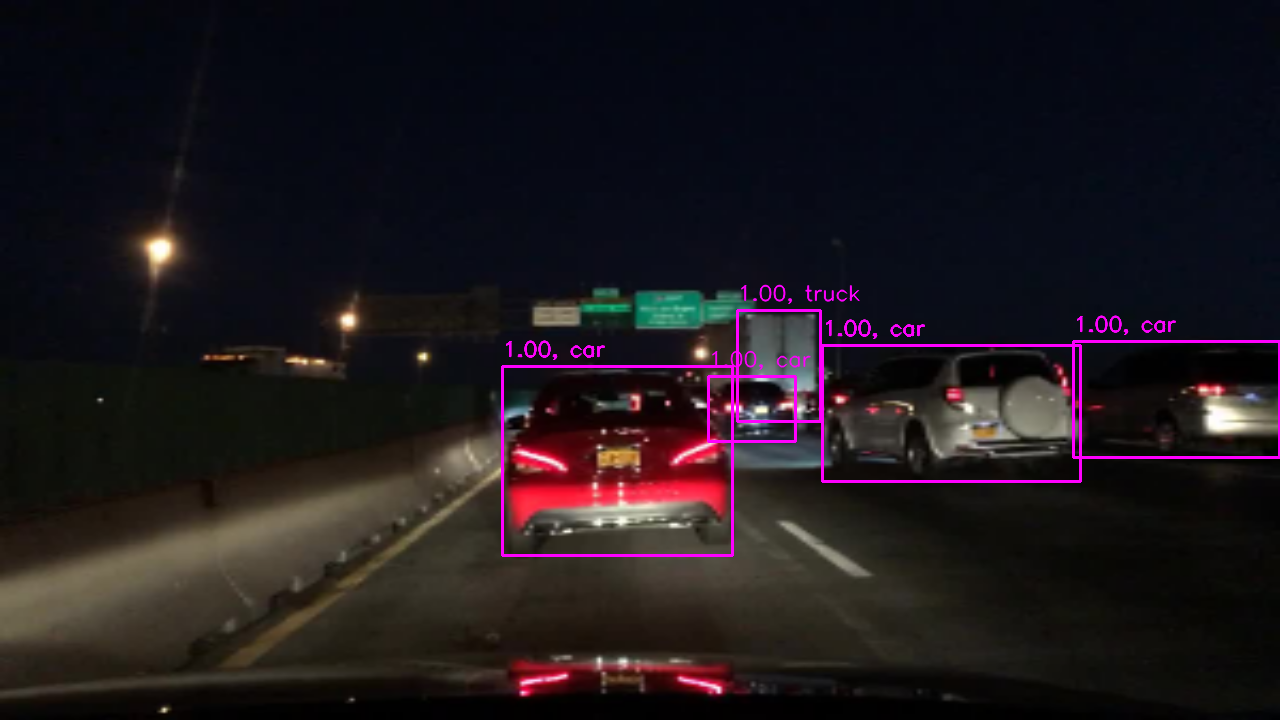
\includegraphics[scale=0.35]{images/dataset_images/9.png}

            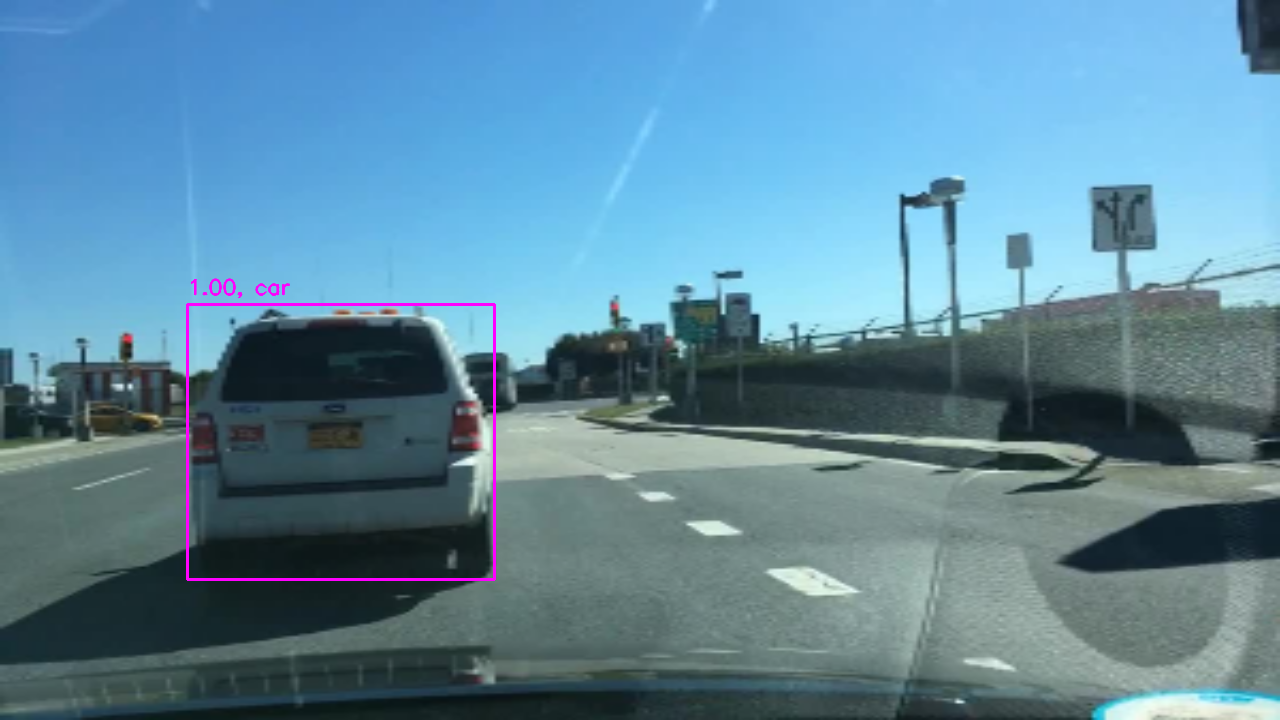
\includegraphics[scale=0.35]{images/dataset_images/10.png}

            \caption[Vanilla prior boxes matched to ground truth]{Image visualizing the matched ground truths to the prior boxes as per the matching strategy established in the SSD's original work by \citet{Liu2016SSDSS}. We can observe that the small object boxes are not matched to the prior boxes resulting in low-quality training data provided.}
            \label{fig:matching strategy basic}
        \end{center}
    \end{figure}
    
    \subsubsection{Results}
    The Average Precision of all the predicted classes from object detection on the test dataset with 10,000 images are presented in Table \ref{map_basic} and the related Precision-Recall (PR) curves are shown in Figure \ref{pr_basic}.
    
    \begin{table}[]
    \renewcommand{\arraystretch}{1.5}
    \caption{Average Precision values of each class in BDD100K dataset using SSD300 model with and without tuned prior boxes}
    \resizebox{\textwidth}{!}{
\scriptsize \begin{tabular}{cllllllllll}

                              &                         & \multicolumn{9}{c}{\textbf{Agents}}  \\ \hline
                              & \multicolumn{1}{l}{\textbf{Models}}         & \multicolumn{1}{l}{\textbf{Pedestrian}} & \multicolumn{1}{l}{\textbf{Rider}} & \multicolumn{1}{l}{\textbf{Car}} & \multicolumn{1}{l}{\textbf{Truck}} & \multicolumn{1}{l}{\textbf{Bus}} & \multicolumn{1}{l}{\textbf{Motorcycle}} & \multicolumn{1}{l}{\textbf{Bicycle}} &\multicolumn{1}{l}{\textbf{Traffic Sign}} & \textbf{mean} \\ \hline
 & \multicolumn{1}{l}{\textbf{SSD300}}         & \multicolumn{1}{l}{0.006}               & \multicolumn{1}{l}{0.004}          & \multicolumn{1}{l}{0.095}        & \multicolumn{1}{l}{0.083}          & \multicolumn{1}{l}{0.15}         & \multicolumn{1}{l}{0.045}               & \multicolumn{1}{l}{0.092}            & \multicolumn{1}{l}{0.001}       &     0.059     \\ \cline{1-11} 
                              & \multicolumn{1}{l}{\textbf{SSD300 - Tuned}} & \multicolumn{1}{l}{0.165}               & \multicolumn{1}{l}{0.135}          & \multicolumn{1}{l}{0.479}        & \multicolumn{1}{l}{0.389}          & \multicolumn{1}{l}{0.389}        & \multicolumn{1}{l}{0.163}               & \multicolumn{1}{l}{0.213}            & \multicolumn{1}{l}{0.186}    &     0.265        \\ \hline
\end{tabular}
        }
        \label{map_basic}
    \end{table}
    
    \begin{figure}
    	\centering
    	\begin{subfigure}[t]{0.325\textwidth}
    		\centering
    		\includegraphics[width=\textwidth]{images/basic_pr/class_pedestrian_pr.jpg}
    		\caption{Pedestrian}
    	\end{subfigure}
    	%
    	\begin{subfigure}[t]{0.325\textwidth}
    		\centering
    		\includegraphics[width=\textwidth]{images/basic_pr/class_rider_pr.jpg}
    		\caption{Rider}
    	\end{subfigure}
    	%
    	\begin{subfigure}[t]{0.325\textwidth}
    		\centering
    		\includegraphics[width=\textwidth]{images/basic_pr/class_car_pr.jpg}
    		\caption{Car}
    	\end{subfigure}
        
    	\begin{subfigure}[t]{0.325\textwidth}
    		\centering
    		\includegraphics[width=\textwidth]{images/basic_pr/class_truck_pr.jpg}
    		\caption{Truck}
    	\end{subfigure}
    	%
    	\begin{subfigure}[t]{0.325\textwidth}
    		\centering
    		\includegraphics[width=\textwidth]{images/basic_pr/class_bus_pr.jpg}
    		\caption{Bus}
    	\end{subfigure}
        %
    	\begin{subfigure}[t]{0.325\textwidth}
    		\centering
    		\includegraphics[width=\textwidth]{images/basic_pr/class_motorcycle_pr.jpg}
    		\caption{Motorcycle}
    	\end{subfigure}
    	
    
    	\begin{subfigure}[t]{0.325\textwidth}
    		\centering
    		\includegraphics[width=\textwidth]{images/basic_pr/class_bicycle_pr.jpg}
    		\caption{Bicycle}
    	\end{subfigure}
        %
    	\begin{subfigure}[t]{0.325\textwidth}
    		\centering
    		\includegraphics[width=\textwidth]{images/basic_pr/class_traffic sign_pr.jpg}
    		\caption{Traffic Sign}
    	\end{subfigure}
    \caption[PR curves with vanilla prior boxes]{Precision recall curves for each class in \acrshort{bdd} dataset}
    \label{pr_basic}
    \end{figure}
    
    \subsubsection{Observations}
    \begin{itemize}
        \item Prior boxes that are tuned for the VOC dataset are not suitable for harder object detection datasets like \acrshort{bdd} or KITTI.
        \item This poor performance of \acrshort{ssd} is attributed to the lack of positively matched ground-truth boxes to the prior boxes resulting in providing poor quality prior boxes for the training of the object detector.
    \end{itemize}

    \subsubsection{Tuning the Prior boxes}
    The above experiment showed that the model's performance is poor because the prior boxes are not tuned correctly.  Hence, the knowledge that is encoded in prior boxes scale and aspect ratios is important for the better performance of \acrshort{ssd} object detection model. The following hyper-parameter changes are done in order to improve the \acrshort{ssd} performance on \acrshort{bdd} dataset:
    \begin{itemize}
        \item From the Figure \ref{fig:OA_EDA} the majority of object that are present in the dataset are very small. Hence, the scale factors $s_{min}$ and $s_{max}$ are reduced so as to match the small object to the prior boxes. The post-tuning scale limits are set to 0.1 and 0.86 respectively.
        \item Adapting to the method proposed by \citet{Liu2016SSDSS}, scales for each prediction layer are set to: $s_1$=0.1, $s_2$=0.29, $s_3$=0.48, $s_4$=0.67, $s_5$ = 0.86. In addition to these scales, we also used a scale of $s_0$=0.05 for Conv4-3 layer inside the VGG-19 network this makes the object detection network to detect small objects.
        \item The scales are set to $a_{r}^{BDD100K} \in (0.5, 1, 1.5, 2, 2.5)$. This selection is done based on the scales of objects in \acrshort{bdd}.
    \end{itemize}
    
    % \begin{figure}
    %     \begin{center}
    %         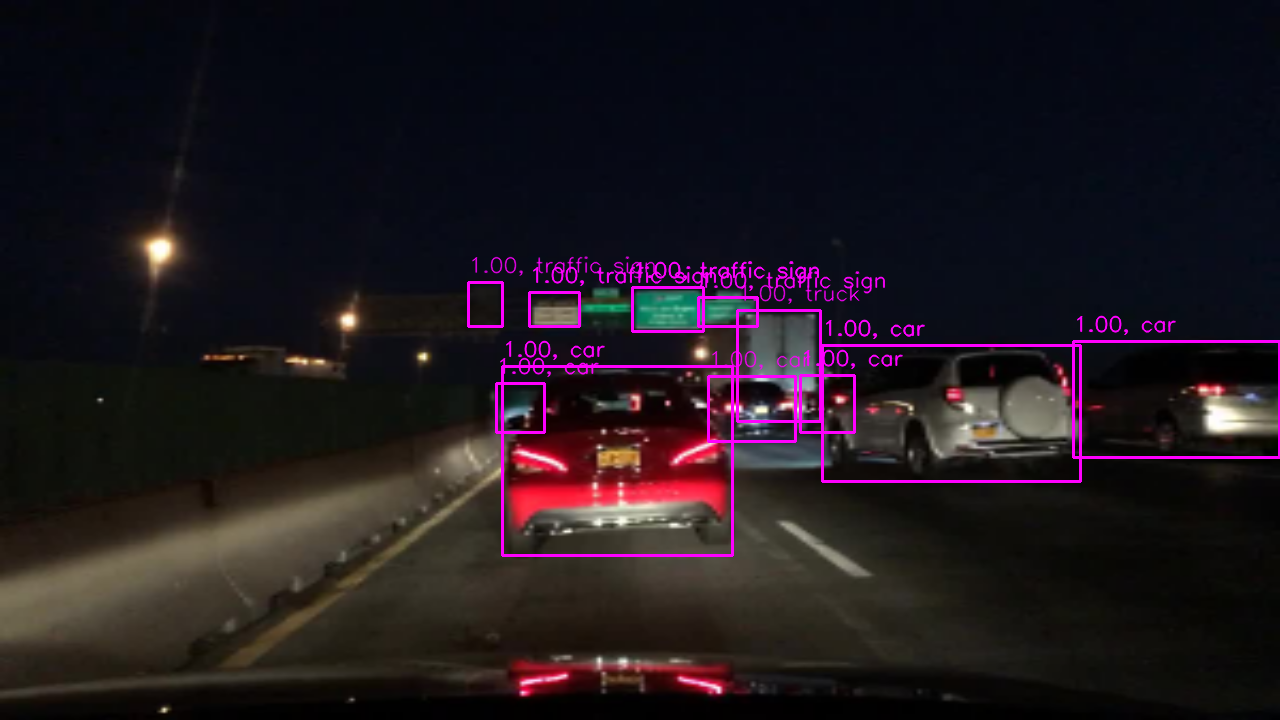
\includegraphics[scale=0.35]{images/dataset_images/tuned_9.png}
        
    %         \vspace{1cm}
        
    %         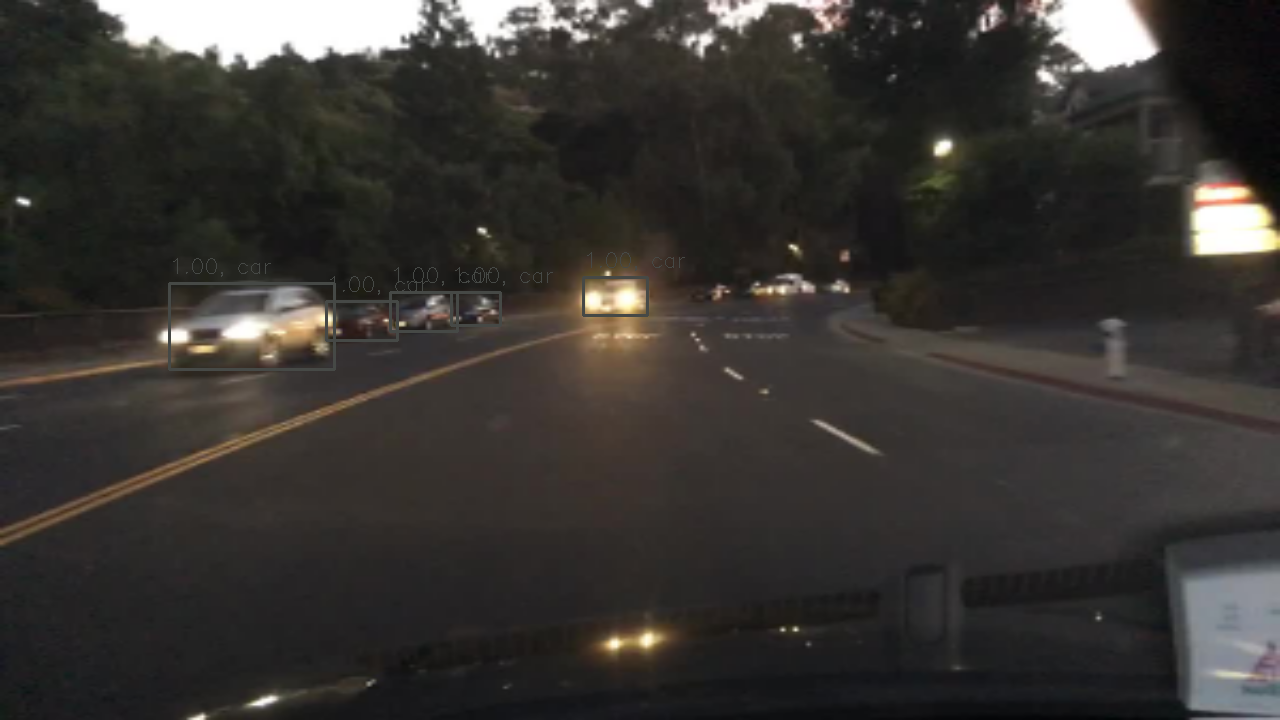
\includegraphics[scale=0.35]{images/dataset_images/tuned_13.png}
    %         \vspace{0.1cm}
    %         \caption{Image showing the matched ground truths to the prior boxes as per the matching strategy established in the SSD's original work by \citet{Liu2016SSDSS} after tuning the prior boxes to encode \acrshort{bdd} specific information. Comparing this Image with Image \ref{fig:matching strategy basic}, we can observe that there is huge increase in the positively matched small boxes count}
    %         \label{fig:matching strategy tuned}
    %     \end{center}
    % \end{figure}
    
    \begin{figure}
        \begin{center}
        \begin{subfigure}[t]{0.9\textwidth}
    		\centering
    		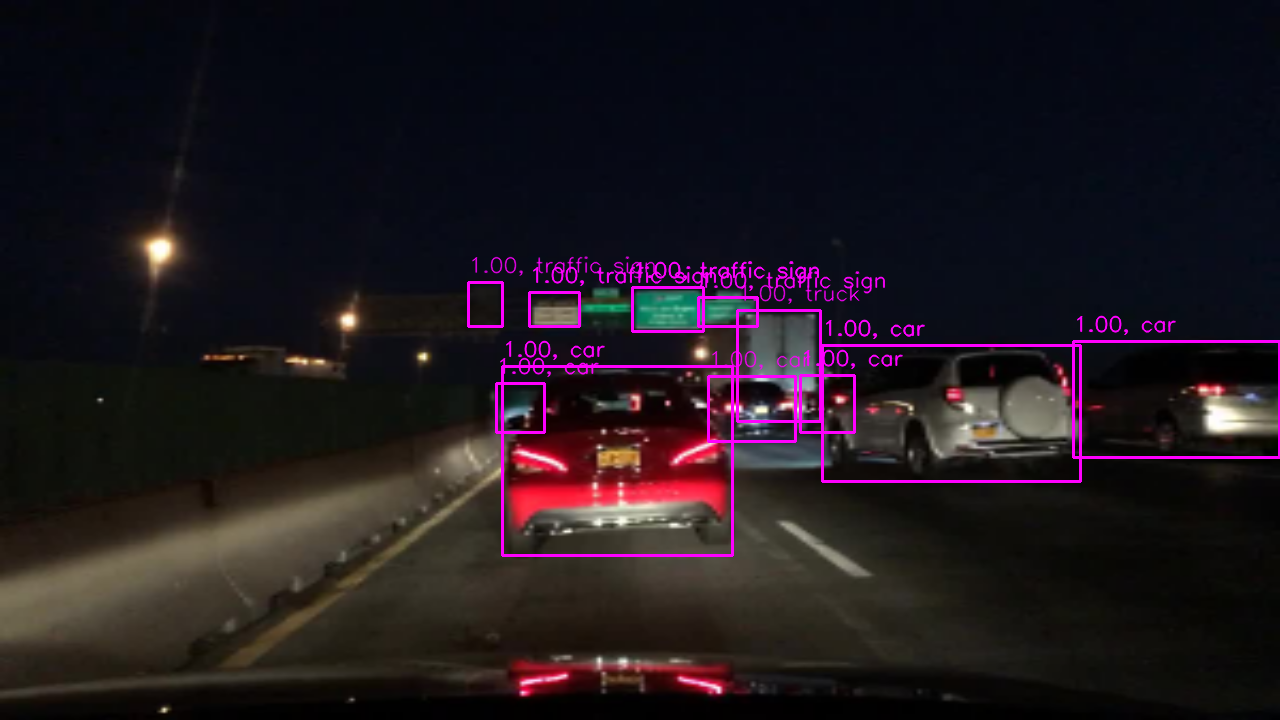
\includegraphics[width=\textwidth]{images/dataset_images/tuned_9.png}
    	\end{subfigure}
    	\end{center}
%     \end{figure}
        	
%   \begin{figure} \ContinuedFloat
    \begin{center}
    	\begin{subfigure}[t]{0.9\textwidth}
    		\centering
    		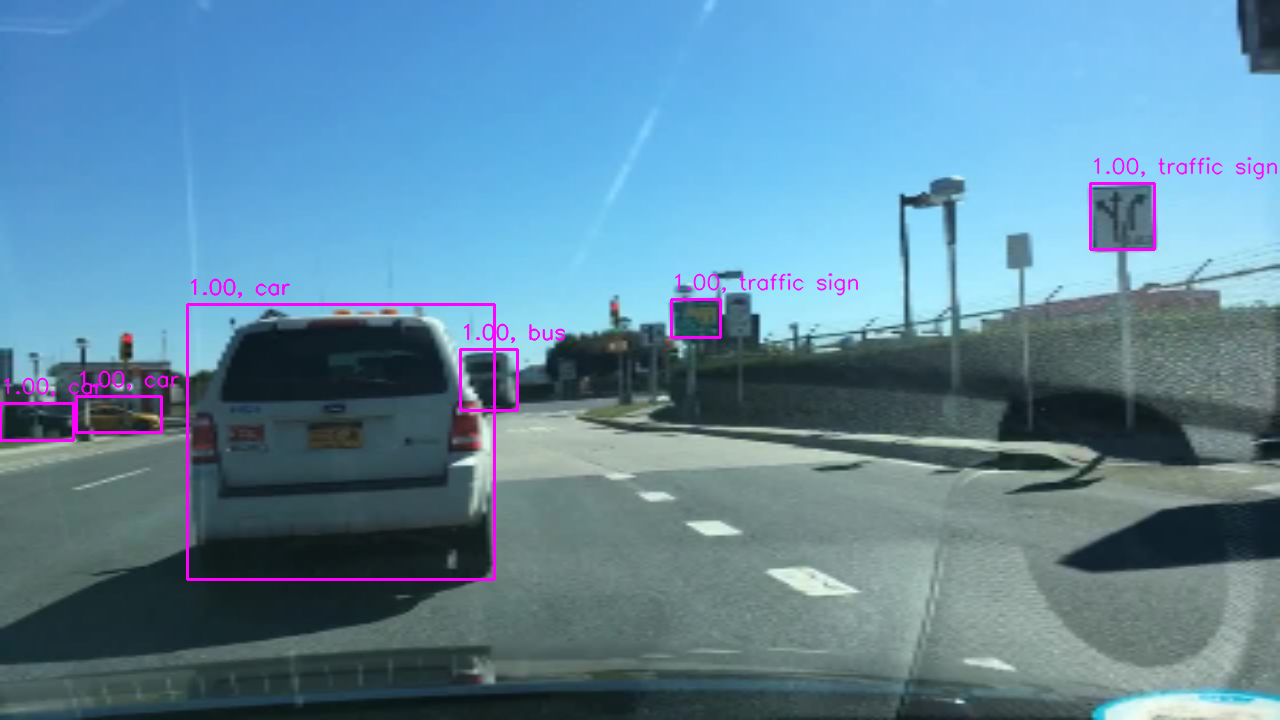
\includegraphics[width=\textwidth]{images/dataset_images/tuned_10.png}
    	\end{subfigure}
            \caption[Tuned prior boxes matched to ground truth]{Image showing the matched ground truths to the prior boxes as per the matching strategy established in the SSD's original work by \citet{Liu2016SSDSS} after tuning the prior boxes to encode \acrshort{bdd} specific information. Comparing this Image with Image \ref{fig:matching strategy basic}, we can observe that there is huge increase in the positively matched ground truth boxes}
            \label{fig:matching strategy tuned}
    \end{center}
    \end{figure}
    
    \begin{figure}
    	\centering
    	\label{fig:pr_basic}
    	\begin{subfigure}[t]{0.325\textwidth}
    		\centering
    		\includegraphics[width=\textwidth]{images/tuned_pr/class_pedestrian_pr.jpg}
    		\caption{Pedestrian}
    	\end{subfigure}
    	%
    	\begin{subfigure}[t]{0.325\textwidth}
    		\centering
    		\includegraphics[width=\textwidth]{images/tuned_pr/class_rider_pr.jpg}
    		\caption{Rider}
    	\end{subfigure}
    	%
    	\begin{subfigure}[t]{0.325\textwidth}
    		\centering
    		\includegraphics[width=\textwidth]{images/tuned_pr/class_car_pr.jpg}
    		\caption{Car}
    	\end{subfigure}
        
    	\begin{subfigure}[t]{0.325\textwidth}
    		\centering
    		\includegraphics[width=\textwidth]{images/tuned_pr/class_truck_pr.jpg}
    		\caption{Truck}
    	\end{subfigure}
    	%
    	\begin{subfigure}[t]{0.325\textwidth}
    		\centering
    		\includegraphics[width=\textwidth]{images/tuned_pr/class_bus_pr.jpg}
    		\caption{Bus}
    	\end{subfigure}
        %
    	\begin{subfigure}[t]{0.325\textwidth}
    		\centering
    		\includegraphics[width=\textwidth]{images/tuned_pr/class_motorcycle_pr.jpg}
    		\caption{Motorcycle}
    	\end{subfigure}
    %     \end{figure}
        	
    % \begin{figure} \ContinuedFloat
        \begin{center}
        	\begin{subfigure}[t]{0.33\textwidth}
        		\centering
        		\includegraphics[width=\textwidth]{images/tuned_pr/class_bicycle_pr.jpg}
        		\caption{Bicycle}
        	\end{subfigure}
            %
        	\begin{subfigure}[t]{0.33\textwidth}
        		\centering
        		\includegraphics[width=\textwidth]{images/tuned_pr/class_traffic sign_pr.jpg}
        		\caption{Traffic Sign}
        	\end{subfigure}
            \caption[PR curves with tuned prior boxes]{Precision recall curves for each class in \acrshort{bdd} dataset with prior boxes tuned using \acrshort{bdd} dataset. We observed a huge increase on the performance of SSD300 model compared to performance shown in Figure \ref{pr_basic}.}
        \end{center}
    \end{figure}
    
    \begin{figure}
        \centering
        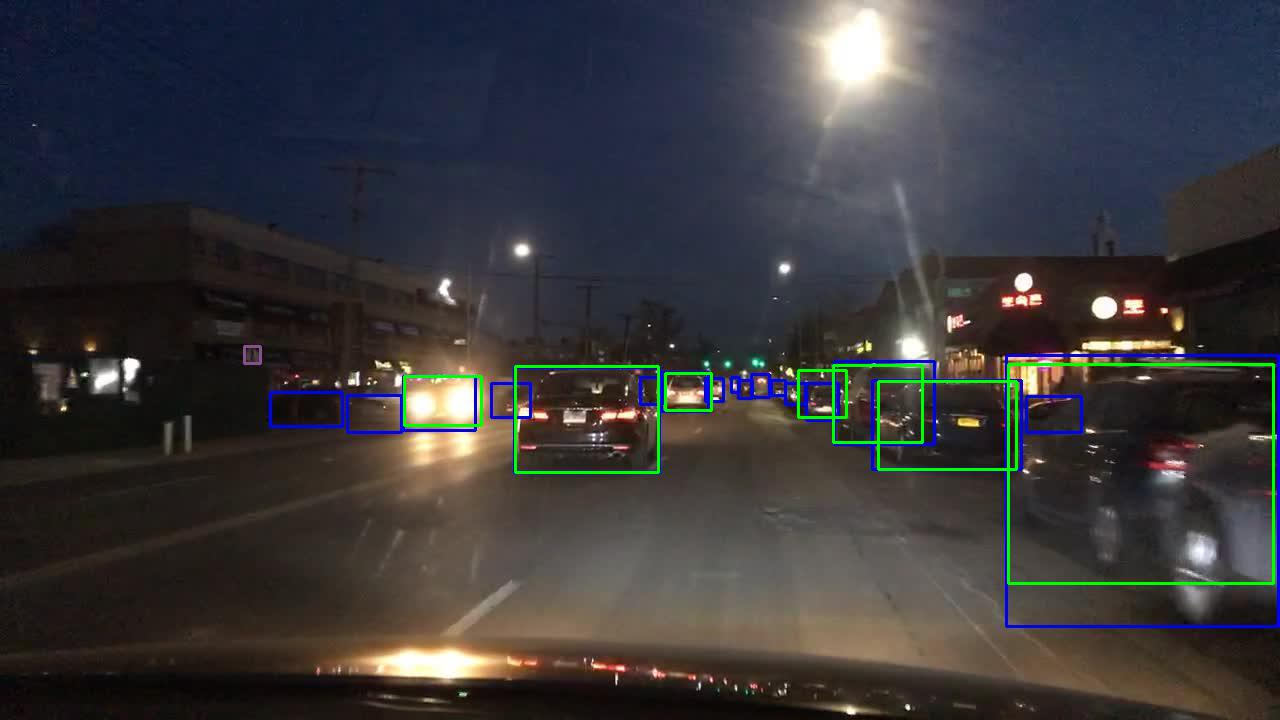
\includegraphics[scale=0.45]{images/detections/ssd/b1d10d08-5b108225.jpg}
        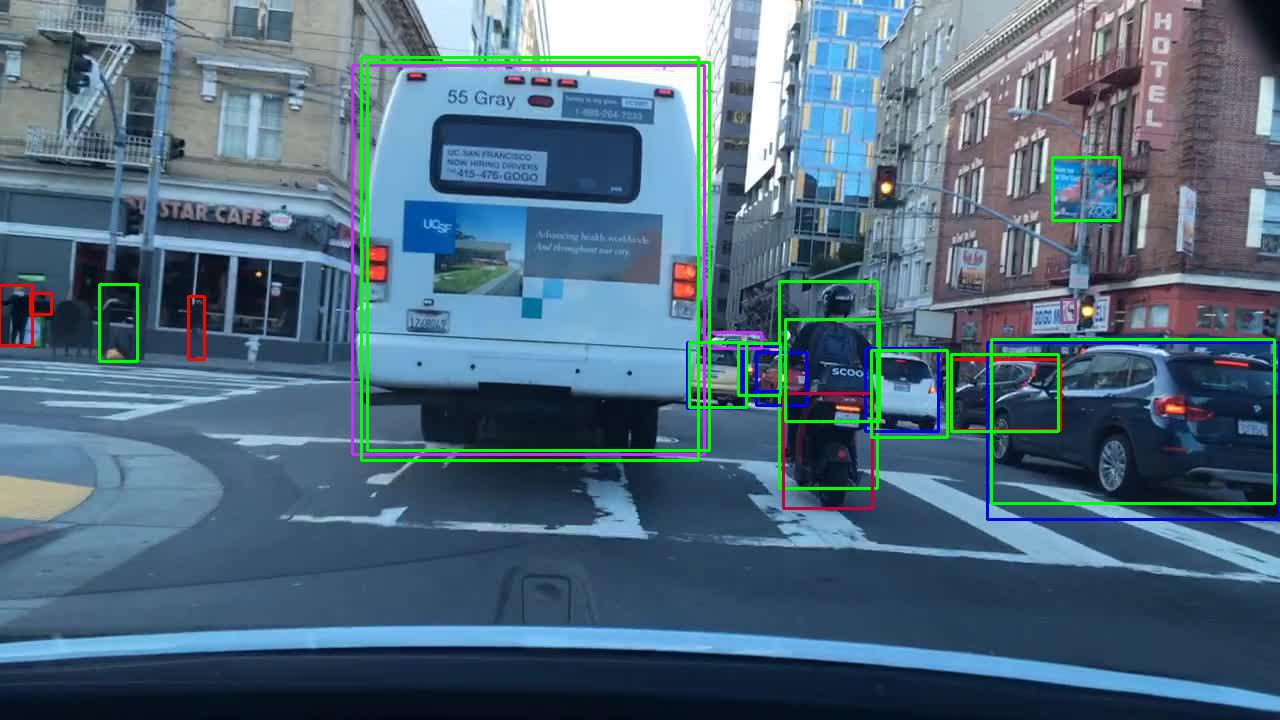
\includegraphics[scale=0.45]{images/detections/ssd/b1d9e136-6c94ea3f.jpg}
        \caption[Detection on images from \acrshort{bdd} dataset]{Detections made by SSD300 model on \acrshort{bdd} dataset. The ground-truth is marked in various different colors other than green and the detected boxes are represented in green. The detector worked well at the night and also detected relatively small objects.}
        \label{fig:bdd_detections}
    \end{figure}
    
    \begin{figure}
        \centering
        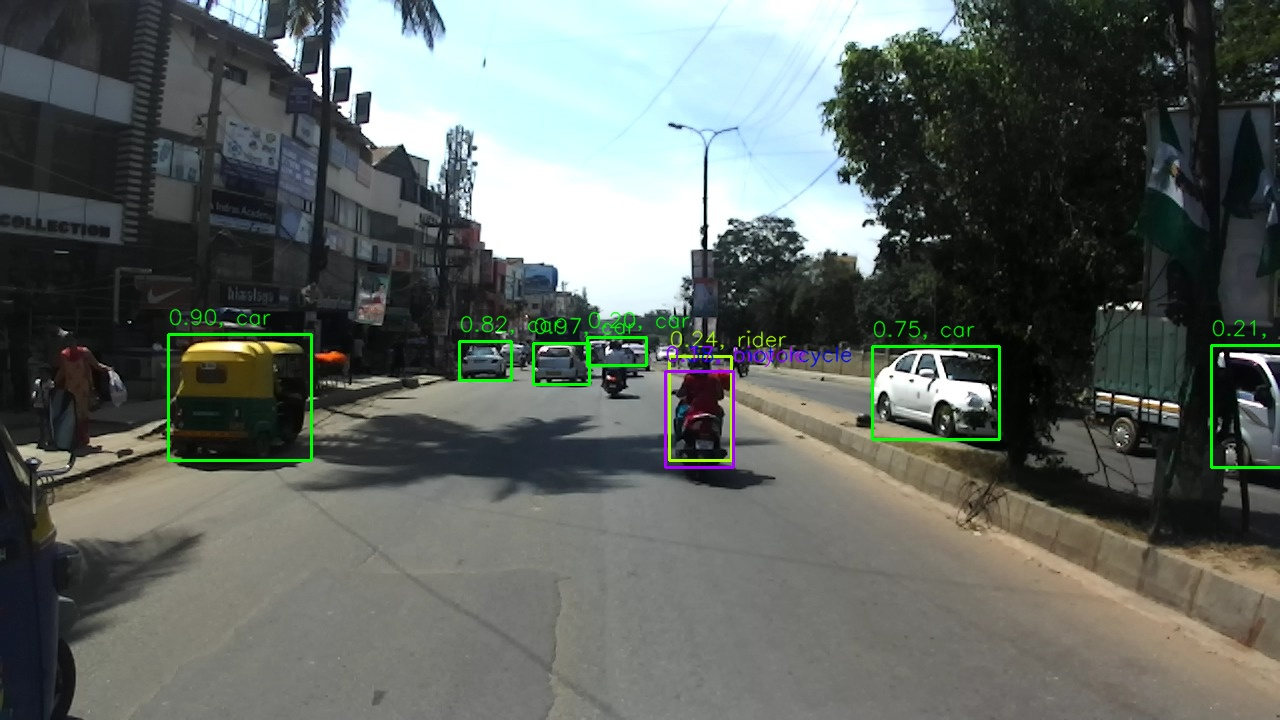
\includegraphics[scale=0.35]{images/det_images/idd_2.jpg}
        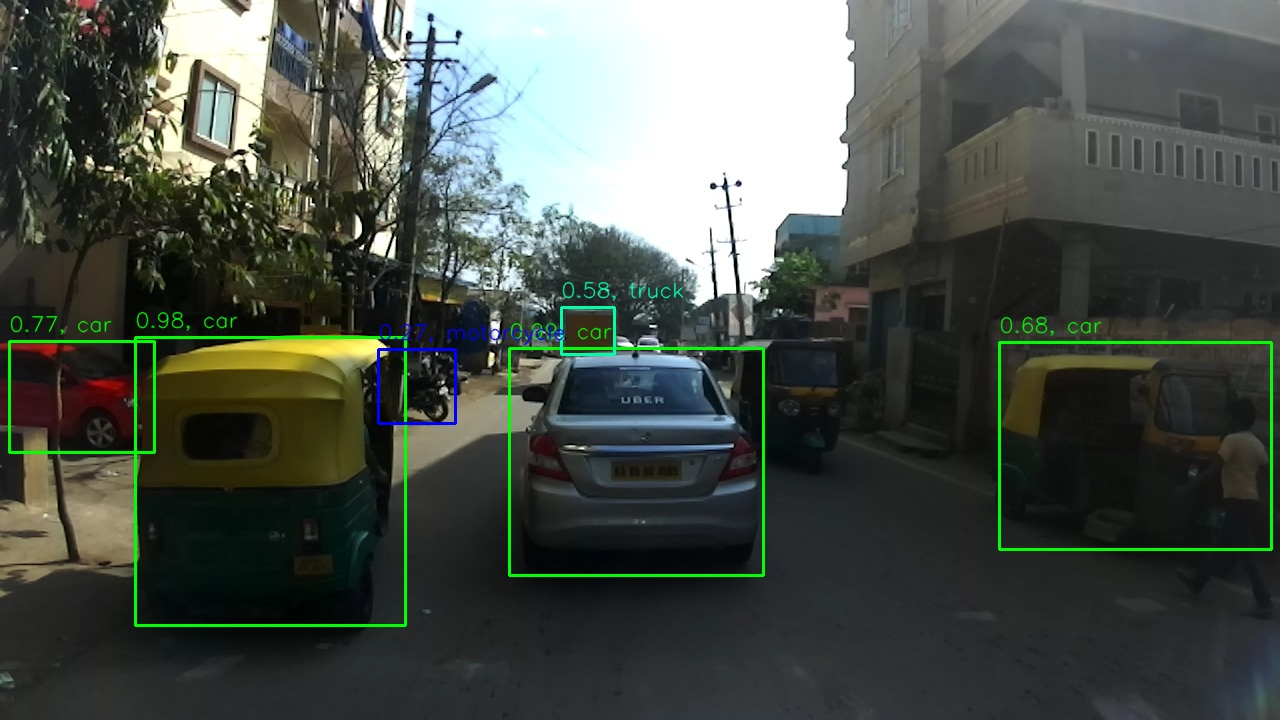
\includegraphics[scale=0.35]{images/det_images/idd_1.jpg}
        \caption[Detection on images from \acrshort{idd} dataset]{Detections made by SSD300 model on \acrshort{idd} dataset. We can observe that the \acrshort{ood} object (Auto-Rickshaw) present in the image is detected and is classified as car with a very high probability of greater than 0.9}
        \label{fig:idd_detection}
    \end{figure}
    
    \subsubsection{Observations}
    \begin{itemize}
        \item We observed an improvement in the performance of the object detection model with proper tuning of prior boxes.
        \item Current \acrshort{ssd} object detector with truncated VGG-19 is comparable to one of the best performing models on the \acrshort{bdd} object detection leader-board.
        \item The object detector model still struggle to detect small objects (Motorcycle, Bicycle, Traffic Sign, Pedestrian) compared to large objects (Car, Truck, Bus). On an average, the average precision values of large objects are 60\% greater than smaller objects.
    \end{itemize}
    % \newpage
    \section{\acrlong{ood} Detection}
    In this Section, we investigate various methods for performing \acrshort{ood} detection. The methods used are Max softmax \cite{hendrycks17baseline}, ODIN \cite{Liang2017} explained in Section \ref{odin_explained} explained in Section \ref{MD_ood} and Uncertainty-based methods \cite{Malinin2018, Oberdiek, Oberdiek2018} using \acrshort{bnn} and Sub-Ensembles for uncertainty quantification. To perfrom this experiments, we use the $OD^{2}$ dataset that is proposed in the Section \ref{Benchmarking}. The performance of the \acrshort{ood} detector is measured using the metrics that are explained in Section \ref{benchmarking_metrics} 
    \subsection{Max Softmax}
    \label{max_softmax_exp}
    The main aim of this experiment is to test the ability of the softmax probability scores from the classification head of the object detector in classifying whether the detection is made from \acrshort{id} and \acrshort{ood} detection. The experiment is performed by posing the \acrshort{ood} detection problem as a classification problem as explained in Section \ref{benchmarking_metrics}. To visualize the ability of max-softmax score to classify \acrshort{bdd}(\acrshort{id}) and \acrshort{idd}(\acrshort{ood}), we use ROC curve as shown in Figure \ref{fig:maxsoftmax_roc} and the \acrlong{auroc} can be used as a comparable metric to other methods.
    
    \begin{figure}
        \centering
        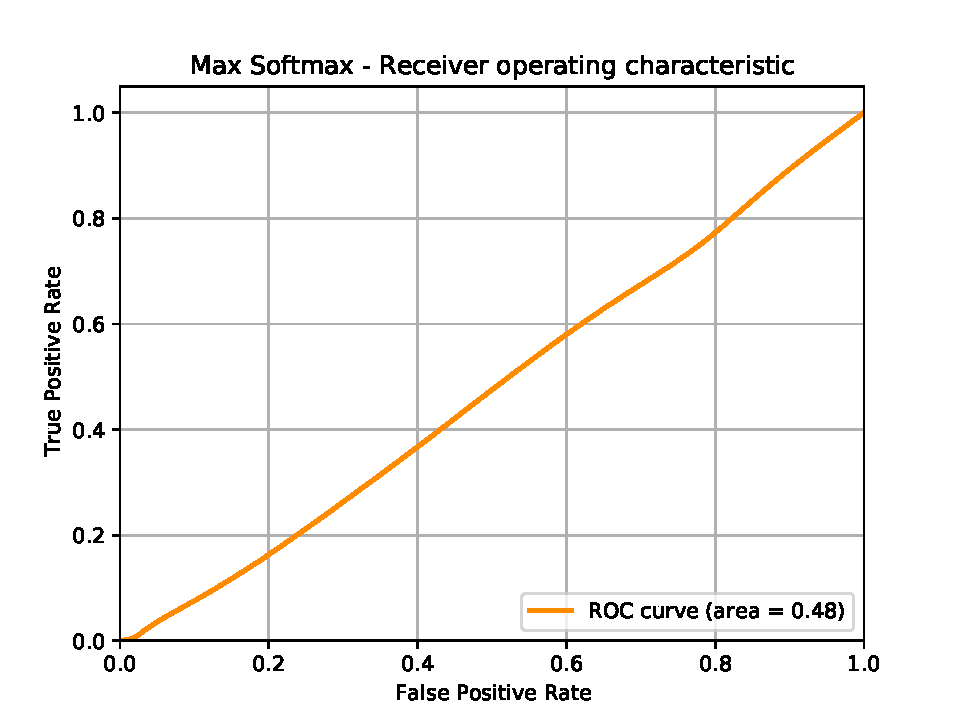
\includegraphics[scale=0.5]{images/ROC/Max Softmax_ROC.pdf}
        \caption[ROC curve for \acrshort{ood} detection using softmax probability score]{ROC curve representing the ability of softmax score in detecting whether the sample is \acrlong{id} or \acrlong{ood}}
        \label{fig:maxsoftmax_roc}
    \end{figure}
    
    Since this is currently used method to decide the models' confidence in its output. The \acrshort{auroc} score produced by this method will be used as a baseline to benchmark the ability of other methods. The results prove that the softmax probability score is not dependable to solve \acrshort{ood} problem. This inability of softmax scores can also be understood from the sample provided in Figure \ref{fig:idd_detection}, in which an \acrshort{ood} sample is assigned a high probability of greater than 0.9.
    
    \subsection{Softmax-based ODIN}
    The main aim of this experiment is to test the ability of ODIN in performing out-of-distribution detection in the case of complex datasets like \acrshort{bdd} and \acrshort{idd}. According to the original work on ODIN, the authors showed that the softmax scores of \acrshort{id} samples are increased at the same time the softmax scores of \acrshort{ood} will have minimum effect on them. This increases the chances of classifying \acrshort{id} and \acrshort{ood} samples using the softmax scores after perturbation.
    \subsubsection{Hyperparameter Optimization}
    As previously mentioned this method introduces two more hyper-parameters, a perturbation magnitude $\epsilon$ and Temperature $T$. From the explanations in Section \ref{odin_explained} we can understand that choosing the best values for these hyperparameters is very important to make a reliable \acrshort{ood} detection possible. Image \ref{fig:perturbed_image} shows different perturbed images with different magnitudes and temperatures.
    
    Since the original work on ODIN is done using very simple classification data the perturbation magnitude and temperature did not work for a complex object detection dataset. Hence, we decided to tune these parameters. To tune these parameters, we performed a grid search over a range of 100 input perturbation magnitude values ranging from 0 to 1, and temperature values are chosen from a set of values from 1 to 1000 at equal intervals are used. The grid search is performed to keep the same performance as with the non-perturbed image, the models' performance is judged by measuring the False Negative (FN) count from the detections. From the extensive search performed, the perturbation magnitude and temperature are set to 0.2 and 1000 respectively.
    
    The \acrshort{roc} curve for classifying \acrshort{bdd} (\acrshort{id}) and \acrshort{idd} (\acrshort{ood}) using the softmax scores after perturbations is visualized in Figure \ref{fig:ODIN_ROC}. 
    
    \begin{figure}
        \centering
        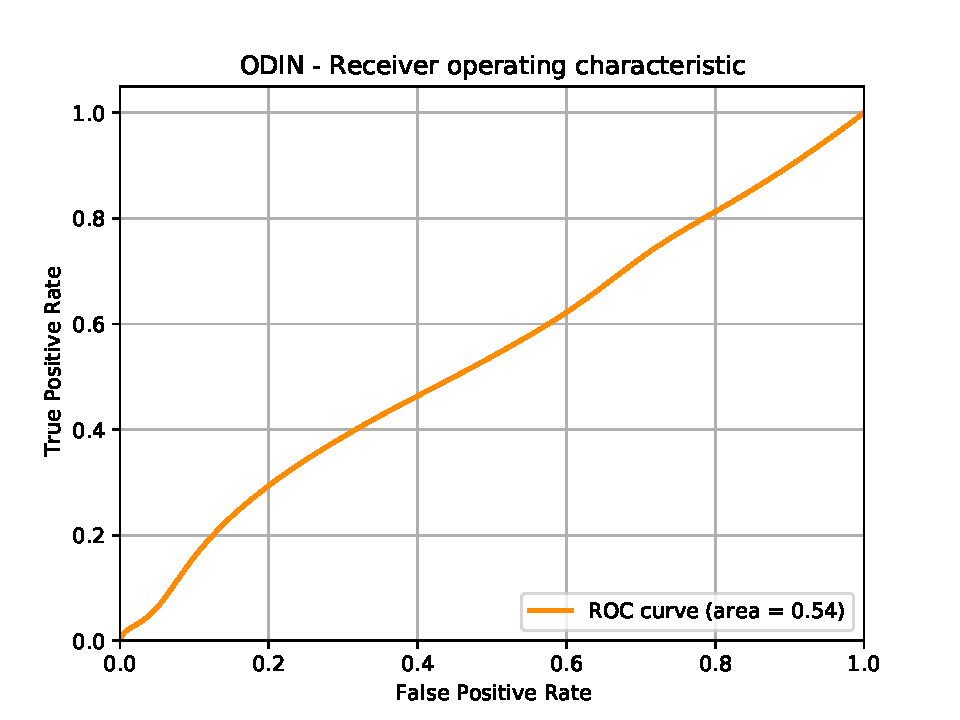
\includegraphics[scale=0.5]{images/ROC/BDD100K vs IDD_ODIN_ROC.pdf}
        \caption[ROC curve for \acrshort{ood} detection using ODIN generated softmax probability score]{ROC curve representing the ability of softmax score after applying temperature scaling and perturbations in detecting whether the sample is \acrlong{id} or \acrlong{ood}. There is a slight increase in \acrshort{auroc} score, but is not significant to improve the safety of the perception systems.}
        \label{fig:ODIN_ROC}
    \end{figure}
    
    \subsubsection{Observations}
    \begin{itemize}
        \item The \acrshort{auroc} score is improved by 12.5\% with applying the perturbation and temperature scaling defined in ODIN compared to the baseline method.
        \item The original work proposed the usage of datasets that are semantically very different and have only one object per image.
        \item In our work, the image has multiple objects with varying sizes resulting in ODIN not being as effective as shown in the original work by the authors.
        \item There is an improvement in \acrshort{ood} detection with the pre-processing of the image using perturbation magnitude and Temperature. But a further increase in the hyper-parameter values resulted in deterioration of object detector performance. 
    \end{itemize}
    \section{Uncertainty based \acrlong{ood} Detection}
    This experiment is aimed at investigating the ability of uncertainty quantification methods using \acrlong{bnn} and Sub-Ensembles in performing \acrshort{ood} samples in the images.
    \subsection{Training Bayesian and Sub-Ensemble based SSD Object Detector}
    \label{exp"uq_methods}
    First, we investigate the ability of \acrshort{bnn} and Sub-Ensemble-based SSD300 object detection model to perform object evaluation and compare their performances with the object detection model evaluated in Section \ref{Exp:1}. From the precision-recall values and curves reported in Table \ref{pr_bnn_subens} and Figures \ref{fig:pr_bnn} and \ref{fig:pr_subens}, we observed that there is a 4.1\% increase in mean average precision values using Bayesian-SSD300 model and a 0.7\% increase in mean average precision values using SubEnsemble-SSD300 model compared to SSD300 model. 
    
    Hence, it can be confirmed that the Bayesian-SSD300 model outperformed the SSD300 and SubEnsemble-SSD300.  These results are also corroborated by the work proposed by \citet{LaBonte2019} to solve the task of segmentation using Flipout sampling-based Bayesian layers, they proved that the bayesian version of their U-Net model had out-performed the normal and ensemble version of their models.
    
    \begin{table}
        \renewcommand{\arraystretch}{1.5}
        \caption{Average Precision values of each class in BDD100K dataset using Bayesian-SSD300 and SubEnsemble-SSD300 models. We observed an increase in performance of the object detector models compared to values reported in Table \ref{map_basic}.}
        \resizebox{\textwidth}{!}{
            \scriptsize \begin{tabular}{lllllllllll}
                                          &                         & \multicolumn{9}{c}{\textbf{Agents}}  \\ \hline
                                          & \multicolumn{1}{l}{\textbf{Models}}         & \multicolumn{1}{l}{\textbf{Pedestrian}} & \multicolumn{1}{l}{\textbf{Rider}} & \multicolumn{1}{l}{\textbf{Car}} & \multicolumn{1}{l}{\textbf{Truck}} & \multicolumn{1}{l}{\textbf{Bus}} & \multicolumn{1}{l}{\textbf{Motorcycle}} & \multicolumn{1}{l}{\textbf{Bicycle}} &\multicolumn{1}{l}{\textbf{Traffic Sign}} & \textbf{Mean} \\ \hline
             & \multicolumn{1}{l}{\textbf{Bayesian - SSD300}}        & \multicolumn{1}{l}{0.172}               & \multicolumn{1}{l}{0.149}          & \multicolumn{1}{l}{0.476}        & \multicolumn{1}{l}{0.4}          & \multicolumn{1}{l}{0.401}         & \multicolumn{1}{l}{0.196}               & \multicolumn{1}{l}{0.232}            & \multicolumn{1}{l}{0.184}       &     0.276     \\ \cline{1-11} 
                                          & \multicolumn{1}{l}{\textbf{SubEnsemble - SSD300}} & \multicolumn{1}{l}{0.167}               & \multicolumn{1}{l}{0.144}          & \multicolumn{1}{l}{0.47}        & \multicolumn{1}{l}{0.393}          & \multicolumn{1}{l}{0.396}        & \multicolumn{1}{l}{0.181}               & \multicolumn{1}{l}{0.211}            & \multicolumn{1}{l}{0.171}    &     0.267        \\ \hline
            \end{tabular}
            }
        \label{pr_bnn_subens}
    \end{table}
    
    \begin{figure}[H]
    	\centering
    	\begin{subfigure}[t]{0.325\textwidth}
    		\centering
    		\includegraphics[width=\textwidth]{images/bnn_pr/class_pedestrian_pr.jpg}
    		\caption{Pedestrian}
    	\end{subfigure}
    	%
    	\begin{subfigure}[t]{0.325\textwidth}
    		\centering
    		\includegraphics[width=\textwidth]{images/bnn_pr/class_rider_pr.jpg}
    		\caption{Rider}
    	\end{subfigure}
    	%
    	\begin{subfigure}[t]{0.325\textwidth}
    		\centering
    		\includegraphics[width=\textwidth]{images/bnn_pr/class_car_pr.jpg}
    		\caption{Car}
    	\end{subfigure}
    	
    % 	\end{figure}
        	
    % \begin{figure}[H] \ContinuedFloat
        
    	\begin{subfigure}[t]{0.325\textwidth}
    		\centering
    		\includegraphics[width=\textwidth]{images/bnn_pr/class_truck_pr.jpg}
    		\caption{Truck}
    	\end{subfigure}
    	%
    	\begin{subfigure}[t]{0.325\textwidth}
    		\centering
    		\includegraphics[width=\textwidth]{images/bnn_pr/class_bus_pr.jpg}
    		\caption{Bus}
    	\end{subfigure}
        %
    	\begin{subfigure}[t]{0.325\textwidth}
    		\centering
    		\includegraphics[width=\textwidth]{images/bnn_pr/class_motorcycle_pr.jpg}
    		\caption{Motorcycle}
    	\end{subfigure}
    
        \begin{center}
    	\begin{subfigure}[t]{0.325\textwidth}
    		\centering
    		\includegraphics[width=\textwidth]{images/bnn_pr/class_bicycle_pr.jpg}
    		\caption{Bicycle}
    	\end{subfigure}
        %
    	\begin{subfigure}[t]{0.325\textwidth}
    		\centering
    		\includegraphics[width=\textwidth]{images/bnn_pr/class_traffic sign_pr.jpg}
    		\caption{Traffic Sign}
    	\end{subfigure}
    \vspace*{-3mm}
    \caption[PR-curves of Bayesian SSD model]{Precision recall curves for each class in \acrshort{bdd} dataset using Bayesian-SSD300 model with prior boxes tuned using \acrshort{bdd} dataset}
    \label{fig:pr_bnn}
    \end{center}
    \end{figure}

    \begin{figure}[H]
    	\centering
    	\begin{subfigure}[t]{0.325\textwidth}
    		\centering
    		\includegraphics[width=\textwidth]{images/sub_ens_pr/class_pedestrian_pr.jpg}
    		\caption{Pedestrian}
    	\end{subfigure}
    	%
    	\begin{subfigure}[t]{0.325\textwidth}
    		\centering
    		\includegraphics[width=\textwidth]{images/sub_ens_pr/class_rider_pr.jpg}
    		\caption{Rider}
    	\end{subfigure}
    	%
    	\begin{subfigure}[t]{0.325\textwidth}
    		\centering
    		\includegraphics[width=\textwidth]{images/sub_ens_pr/class_car_pr.jpg}
    		\caption{Car}
    	\end{subfigure}
    	
    		 \end{figure}
        	
    \begin{figure}[ht] \ContinuedFloat
        
    	\begin{subfigure}[t]{0.325\textwidth}
    		\centering
    		\includegraphics[width=\textwidth]{images/sub_ens_pr/class_truck_pr.jpg}
    		\caption{Truck}
    	\end{subfigure}
    	%
    	\begin{subfigure}[t]{0.325\textwidth}
    		\centering
    		\includegraphics[width=\textwidth]{images/sub_ens_pr/class_bus_pr.jpg}
    		\caption{Bus}
    	\end{subfigure}
        %
    	\begin{subfigure}[t]{0.325\textwidth}
    		\centering
    		\includegraphics[width=\textwidth]{images/sub_ens_pr/class_motorcycle_pr.jpg}
    		\caption{Motorcycle}
    	\end{subfigure}
    	
    
   
        \begin{center}
    	\begin{subfigure}[t]{0.325\textwidth}
    		\centering
    		\includegraphics[width=\textwidth]{images/sub_ens_pr/class_bicycle_pr.jpg}
    		\caption{Bicycle}
    	\end{subfigure}
        %
    	\begin{subfigure}[t]{0.325\textwidth}
    		\centering
    		\includegraphics[width=\textwidth]{images/sub_ens_pr/class_traffic sign_pr.jpg}
    		\caption{Traffic Sign}
    	\end{subfigure}
    	\end{center}
        \vspace*{-3mm}
        \caption[PR curves of Sub-Ensemble based SSD300 model]{Precision recall curves for each class in \acrshort{bdd} dataset using SubEnsemble-SSD300 model with prior boxes tuned using \acrshort{bdd} dataset}
        \label{fig:pr_subens}
    \end{figure}
    \newpage
    \subsection{Quantification of Uncertainty in SSD Object Detector}
    \label{uq_methods}
    To quantify the uncertainty in the detection made by \acrshort{ssd}, we measure the probability score, entropy and bounding box deviation from all the 8732 detection boxes regressed by the object detection model.
    \subsubsection{Probability}
    Though we already used probability scores to evaluate \acrshort{ood} detection ability in Section \ref{max_softmax_exp} but the previous work done on uncertainty quantification methods \cite{Blundell2015, shridhar2019comprehensive, gal2016uncertainty} showed that the softmax scores extracted as explained in Section \ref{prob_entropy_calc} proved to be effective in resulting a robust softmax scores for samples unknown to the trained model. Figure \ref{fig:bnn_prob_summary} shows the summary of the probability scores produced on both \acrshort{bdd} and \acrshort{idd} dataset.
    \begin{figure}[H]
        \centering
        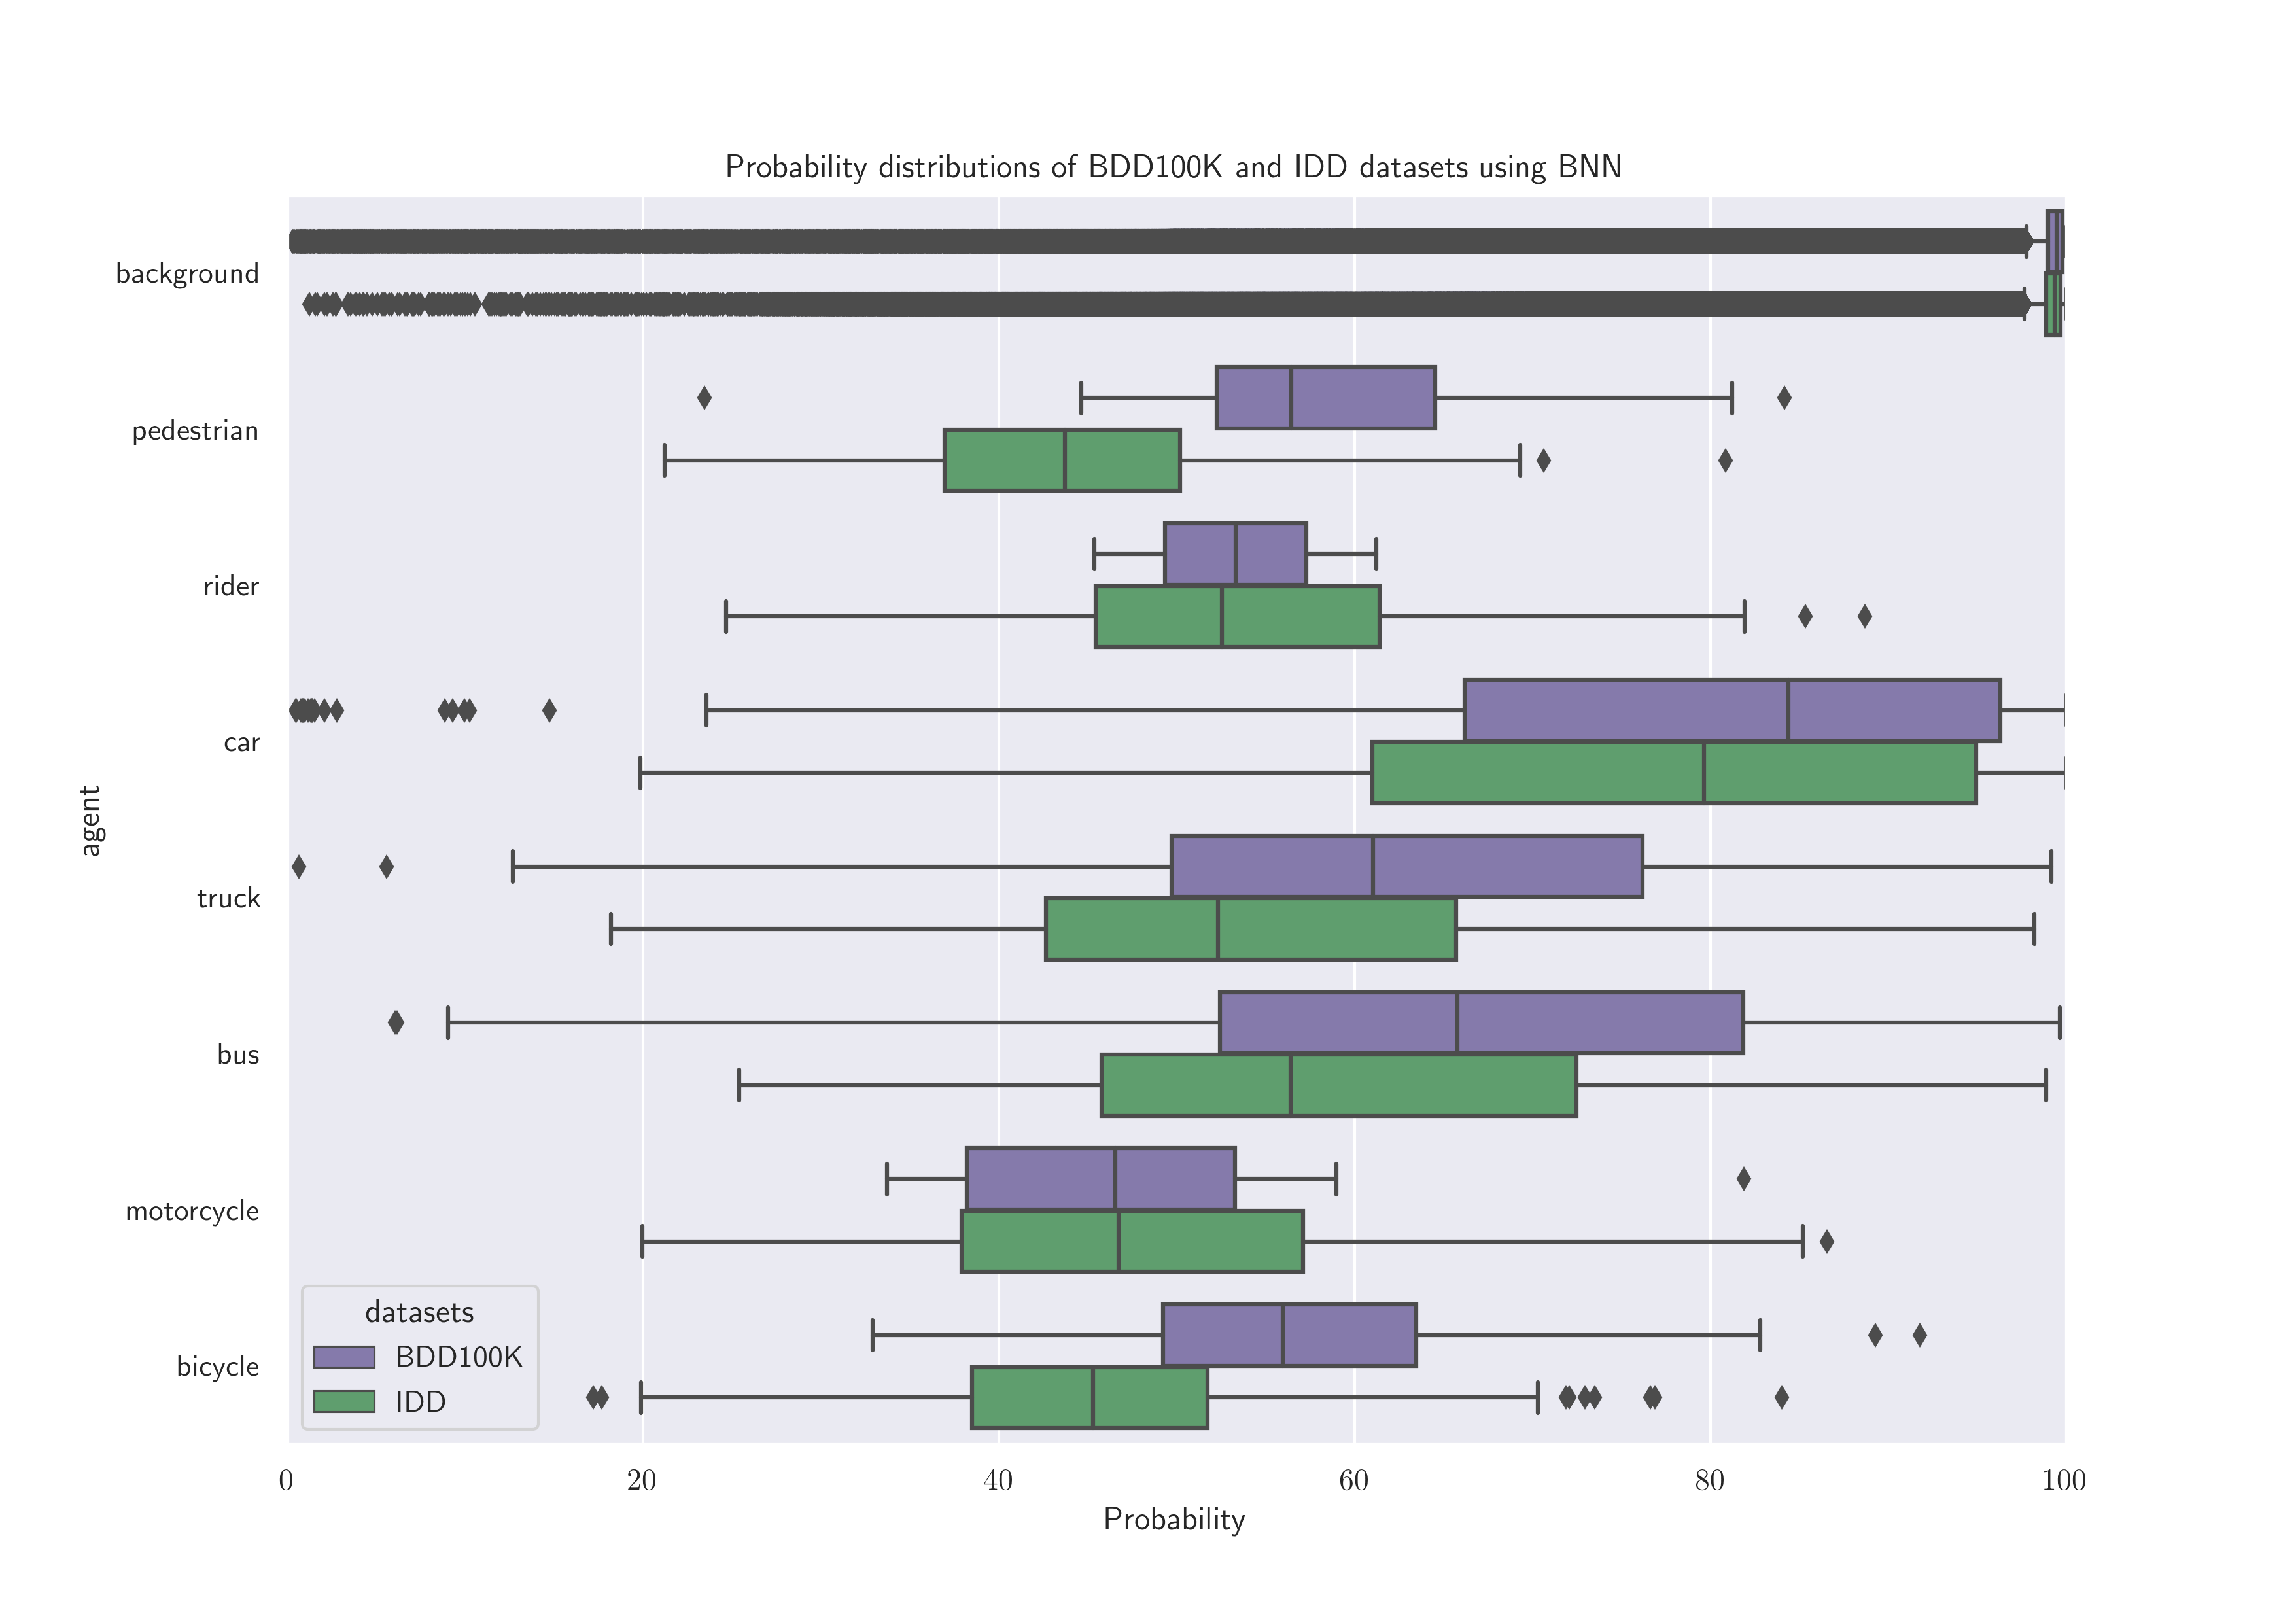
\includegraphics[scale=0.6]{images/distributions/BNN_bdd_vs_iid_probabilities.png}
        \caption[Box plot of probability with Bayesian model]{Box plot representing the summary of the probability calculated as the mean of the softmax scores from all the forward passes through the \acrshort{bnn}}
        \label{fig:bnn_prob_summary}
    \end{figure}
    
    \begin{figure}[H]
        \centering
        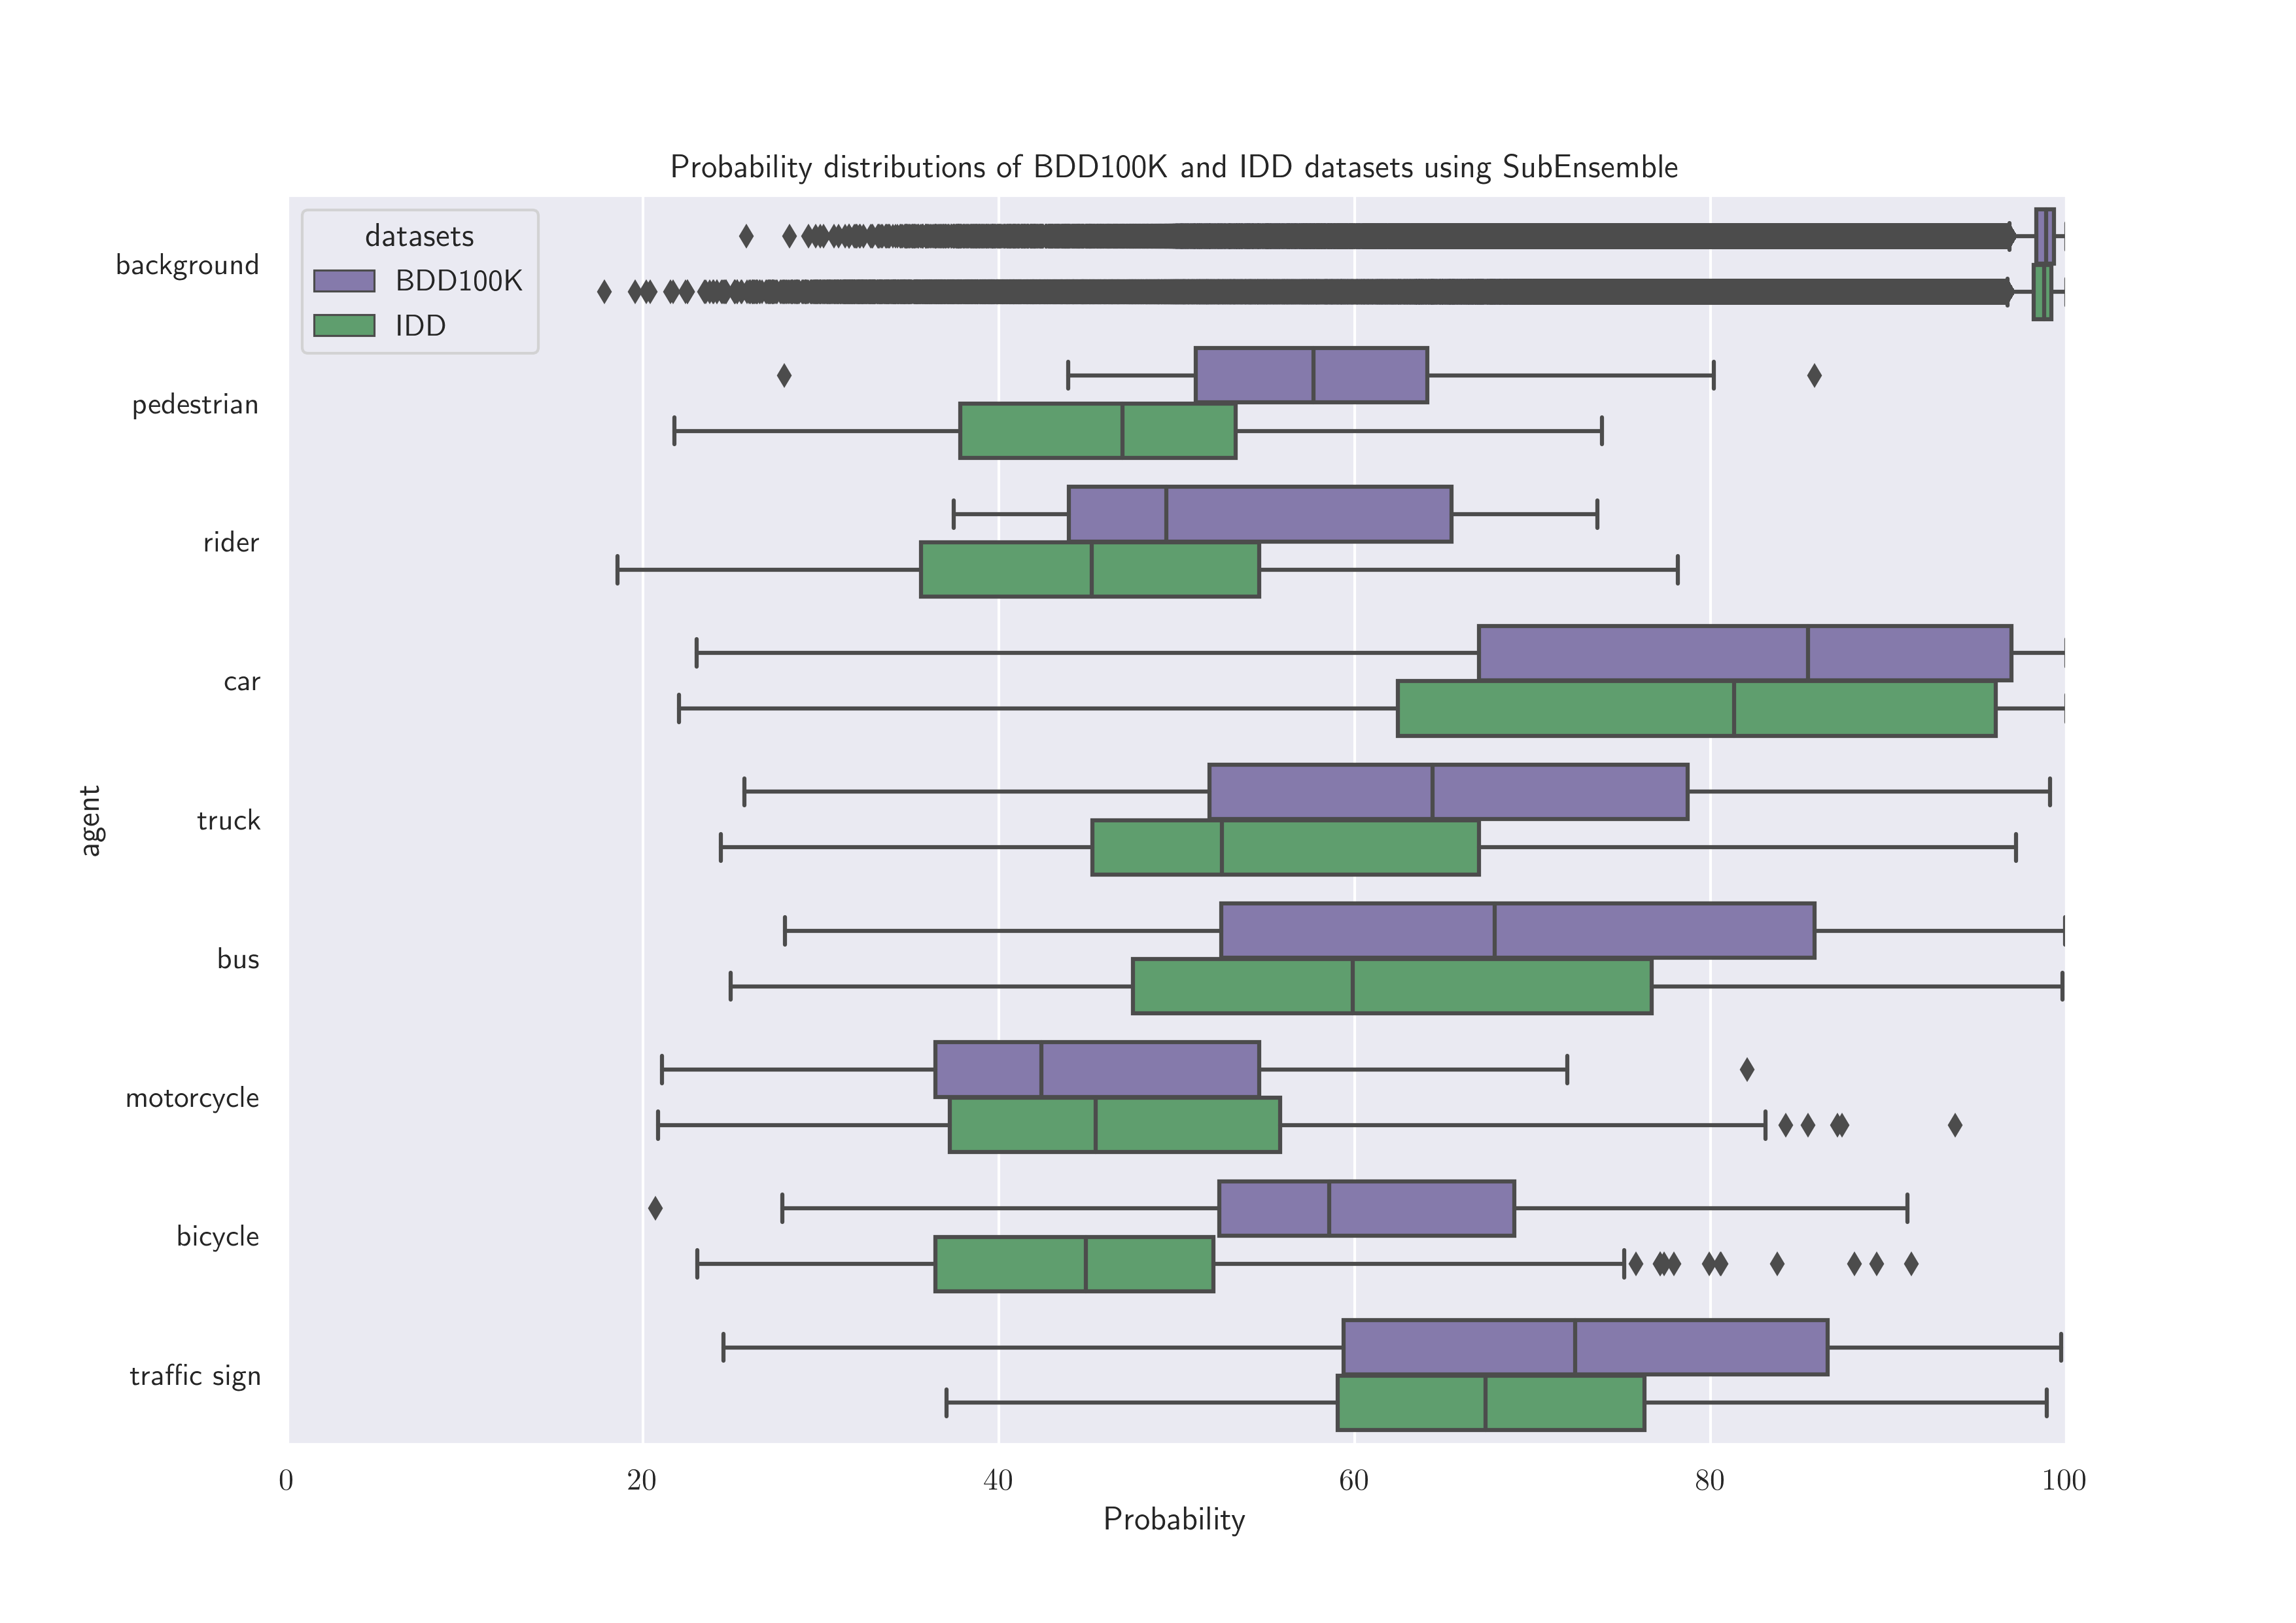
\includegraphics[scale=0.6]{images/distributions/SubEns_bdd_vs_iid_probabilities.png}
        \caption[Box plot of probability with Sub-Ensemble model]{Box plot representing the summary of the probability calculated as the mean of the softmax scores from all the models in the Sub-Ensemble network}
        \label{fig:subens_prob_summary}
    \end{figure}
    
    Our observations from the probability information shown in Figure \ref{fig:bnn_prob_summary} and Figure \ref{fig:subens_prob_summary} are:
    \begin{itemize}
        \item The softmax scores for detections from \acrshort{bdd} dataset are in general greater than the detections from \acrshort{idd} dataset.
        \item Softmax scores of background class are high because both \acrshort{bdd} dataset and \acrshort{idd} dataset belong to the driving domain.
        \item It can be observed that the most similar object in \acrshort{bdd} and \acrshort{idd} datasets like car and motorcycle has almost similar softmax score distributions.
        \item Since the number of traffic signs detected by \acrshort{bnn} in \acrshort{idd} dataset are \textbf{\textit{Zero}}, We decided not to consider the class for benchmarking purposes using \acrshort{bnn}.
        
    \end{itemize}
    
    \subsubsection{Entropy}
    The entropy of detection is calculated from the mean softmax scores as mentioned in Section \ref{prob_entropy_calc}. According to previous work proposed by \citet{Ovadia2019} used uncertainty in detecting \acrshort{ood} samples to solve classification tasks, the entropy is high in case of \acrshort{ood} samples.
    
    \begin{figure}[ht]
        \centering
        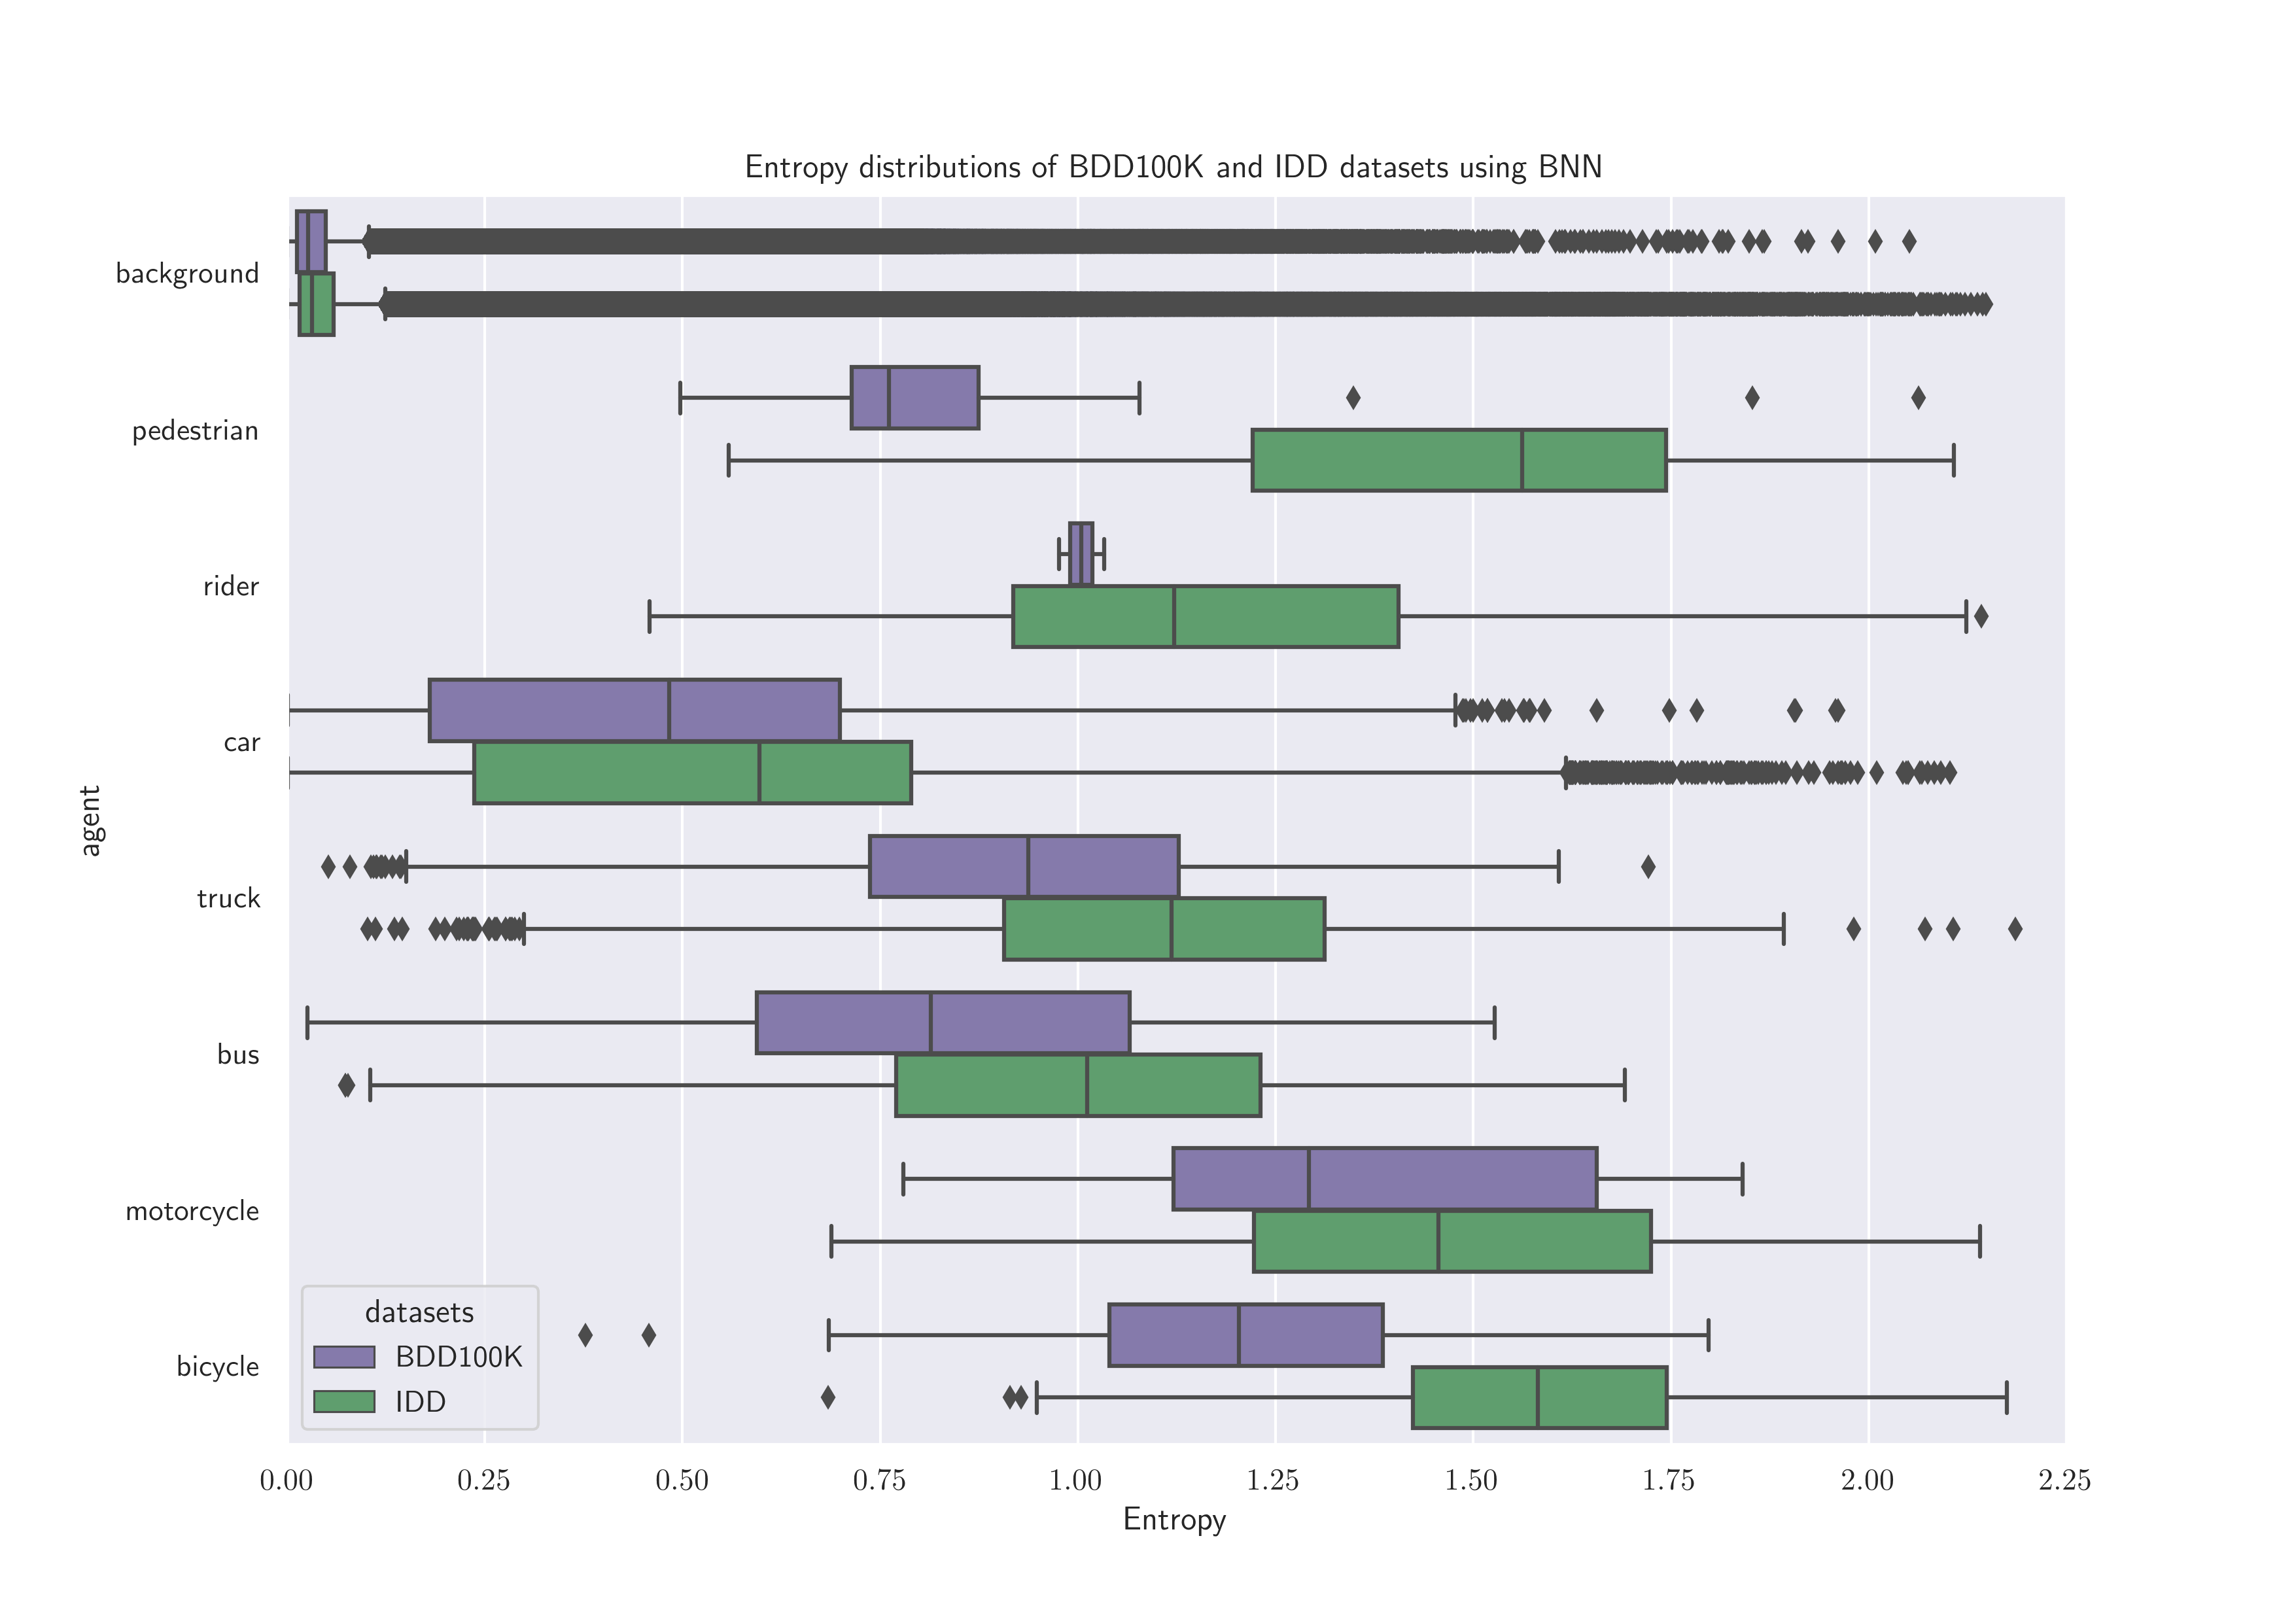
\includegraphics[scale=0.55]{images/distributions/BNN_bdd_vs_iid_entropy.png}
        \caption[Box plot of entropies with Bayesian model]{Box plot representing the summary of the entropy calculated from the mean of the softmax scores from all the forward passes through the \acrshort{bnn}}
        \label{fig:bnn_ent_summary}
    \end{figure}
    
    \begin{figure}[ht]
        \centering
        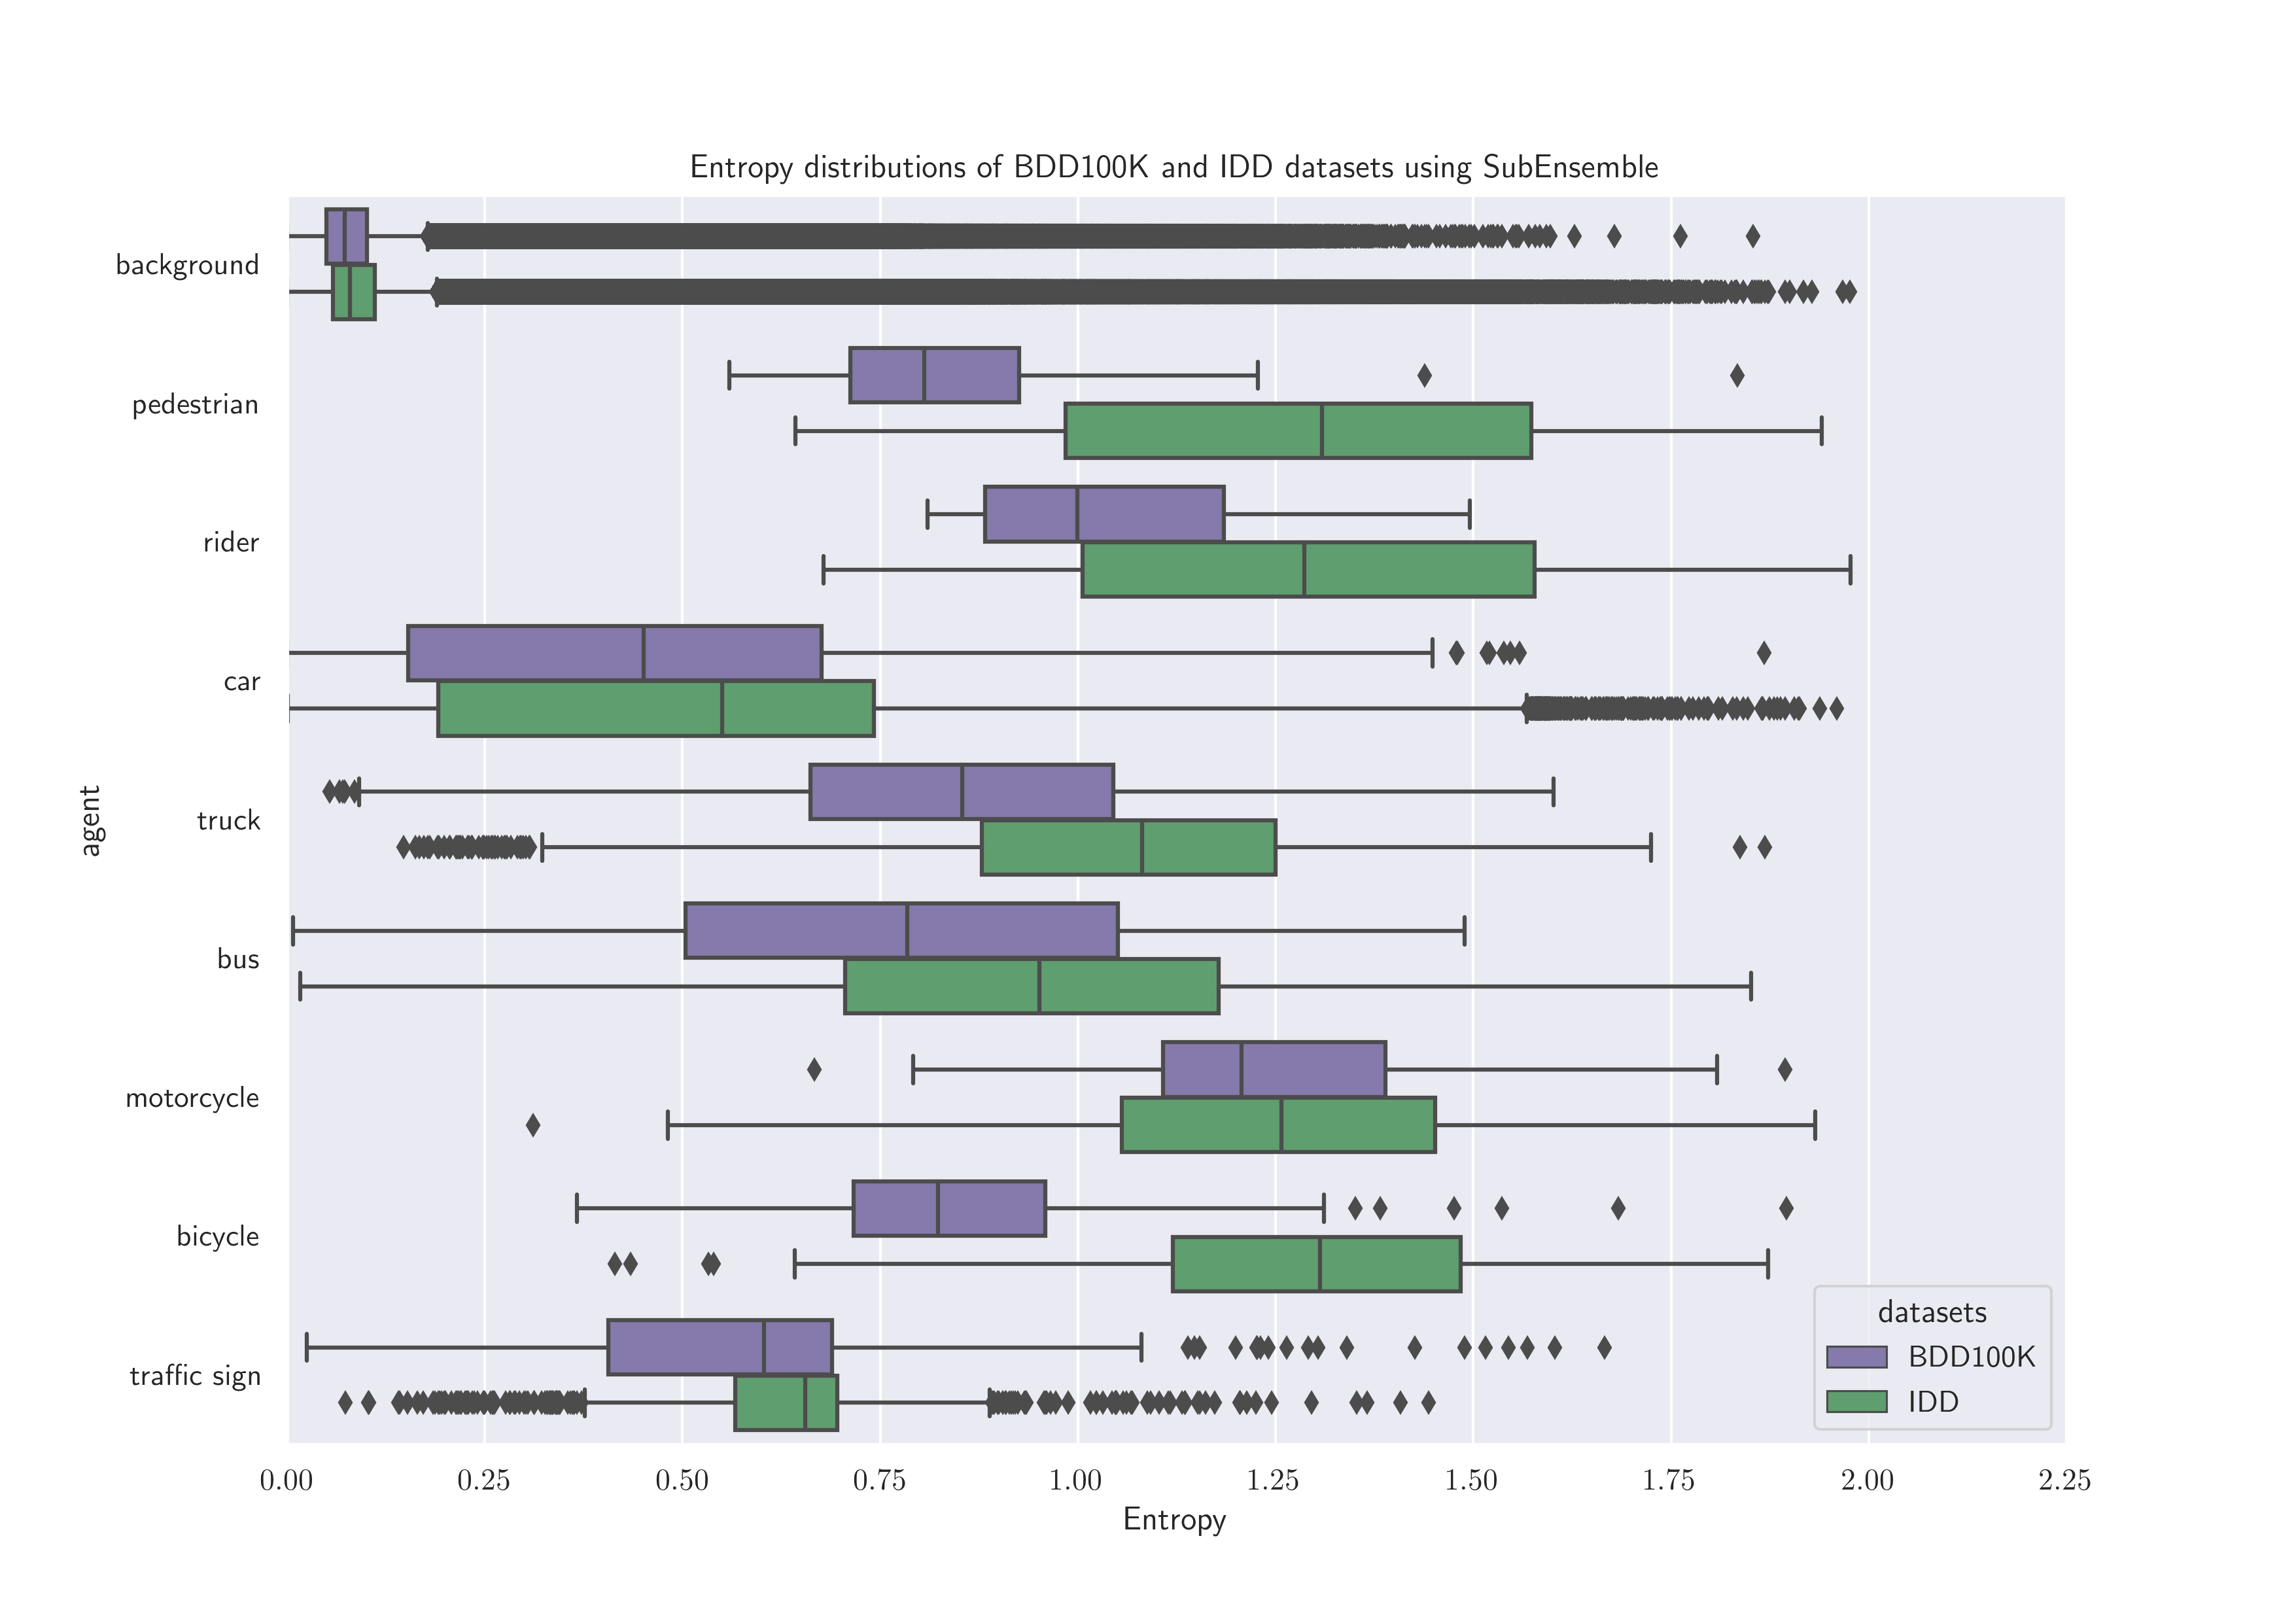
\includegraphics[scale=0.55]{images/distributions/SubEns_bdd_vs_iid_entropy.png}
        \caption[Box plot of entropies with Sub-Ensemble model]{Box plot representing the summary of the entropy calculated from the mean of the softmax scores from all the models in the Sub-Ensemble networks}
        \label{fig:subens_ent_summary}
    \end{figure}
    
    From the Figure \ref{fig:bnn_ent_summary} and Figure \ref{fig:subens_ent_summary} which depicts the information about the distribution of entropies from the inferences made by the \acrshort{bnn}. The key observations are:
    
    \begin{itemize}
        \item Entropy differentiates the \acrshort{bdd} and \acrshort{idd} data better than probability scores.
        \item The information presented also shows that entropy cannot differentiate the \acrshort{bdd} and \acrshort{idd} datasets. This is due to the samples from \acrshort{idd} datasets are ambiguous compared to \acrshort{bdd} dataset. 
        \item Entropy is inherently not able to differentiate aleatoric uncertainty of ambiguous \acrshort{ood} samples and the epistemic uncertainty of pure \acrshort{ood} samples. This result is with the results from the work proposed by \citet{kirsch2021pitfalls}. The results show that entropy is not a good measure in detecting \acrshort{ood} samples which are dominated by ambiguous samples.
    \end{itemize}
    
    
    \subsubsection{Box Deviation}
    Box Deviation is calculated as mentioned in Section \ref{bdev_calc}. This quantifies the inherent uncertainty in the regression head of the \acrshort{ssd} object detection network. The bounding box deviations of both \acrshort{bdd} and \acrshort{idd} datasets are shown in Figures \ref{fig:bnn_dev_summary} and \ref{fig:subens_dev_summary}.
    
    From the Figures \ref{fig:bnn_dev_summary} and \ref{fig:subens_dev_summary}, we inferred that
    \begin{itemize}
        \item The distribution of box deviations is almost similar for both SubEnsembles and \acrshort{bnn}.
        \item \acrshort{bnn} produced higher box deviation values than Sub-Ensembles.
        \item The box deviations showed a higher ability of differentiation between \acrshort{bdd} and \acrshort{idd} dataset.
    \end{itemize}
    
    \begin{figure}[H]
        \centering
        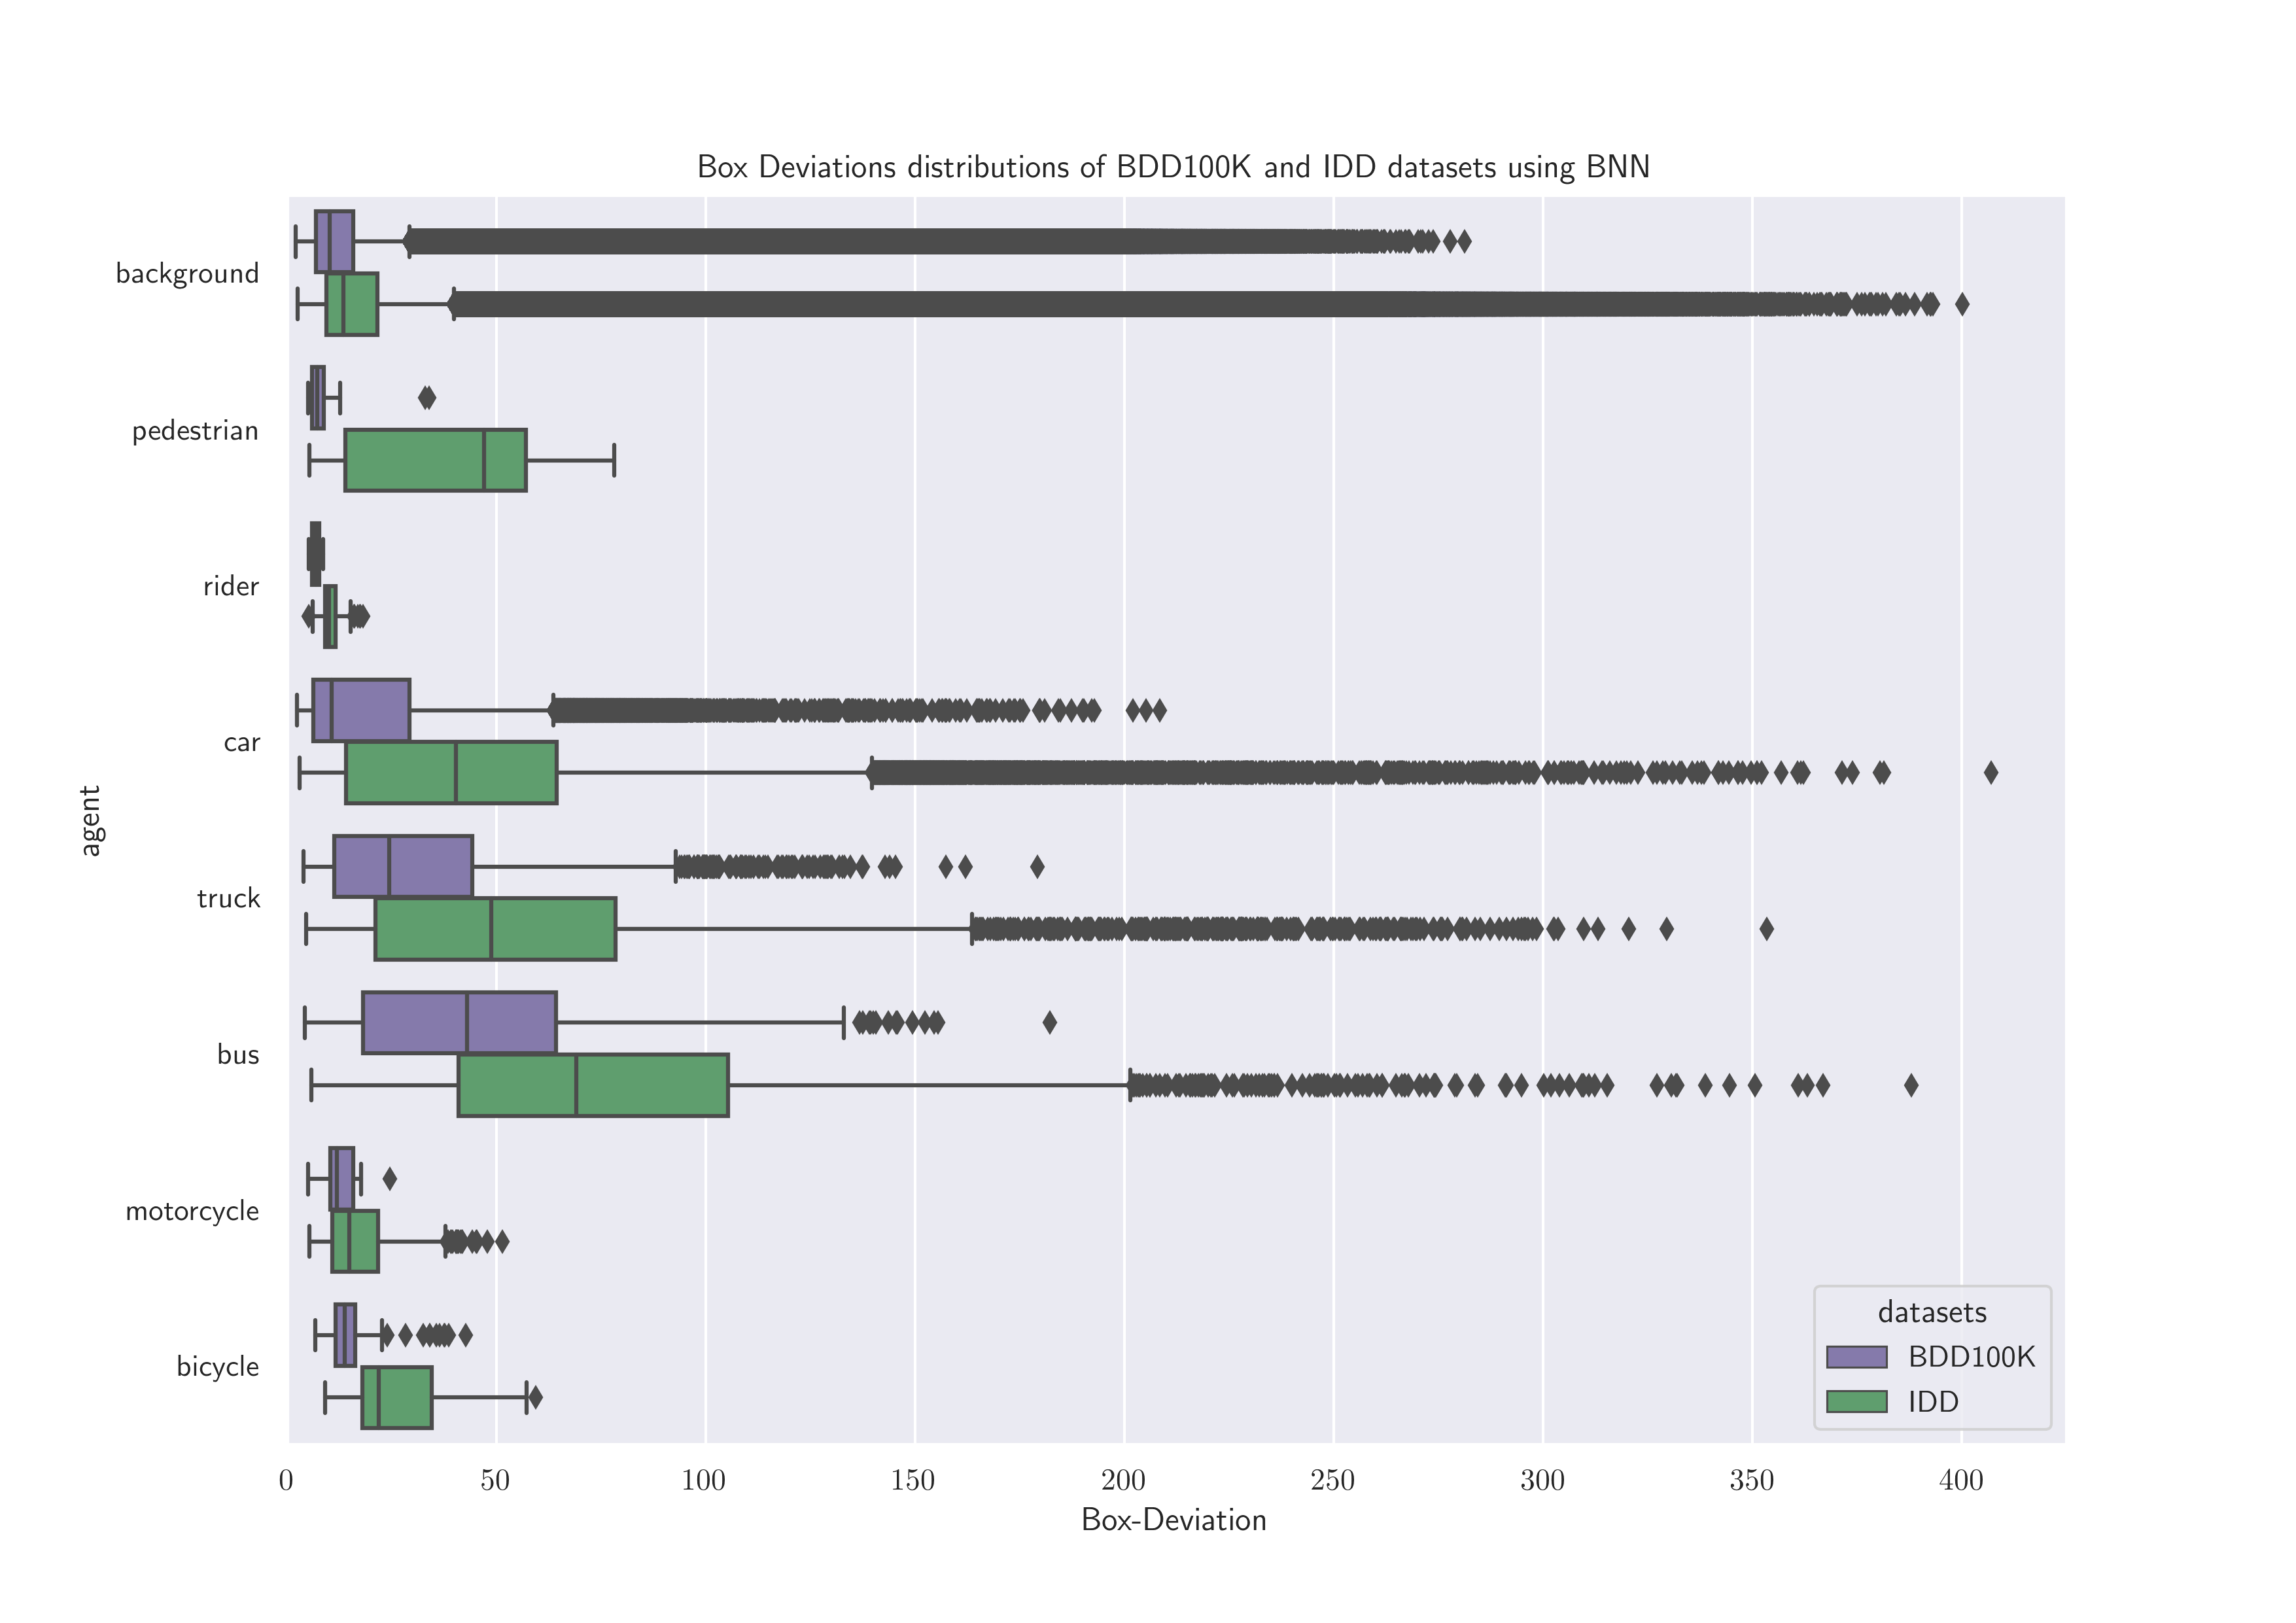
\includegraphics[scale=0.6]{images/distributions/BNN_bdd_vs_iid_deviations.png}
        \caption[Box plot of box deviations with Bayesian model]{Box plot representing the summary of the box deviations calculated using the box detections from all the forward passes through the \acrshort{bnn}}
        \label{fig:bnn_dev_summary}
    \end{figure}
    \begin{figure}[H]
        \centering
        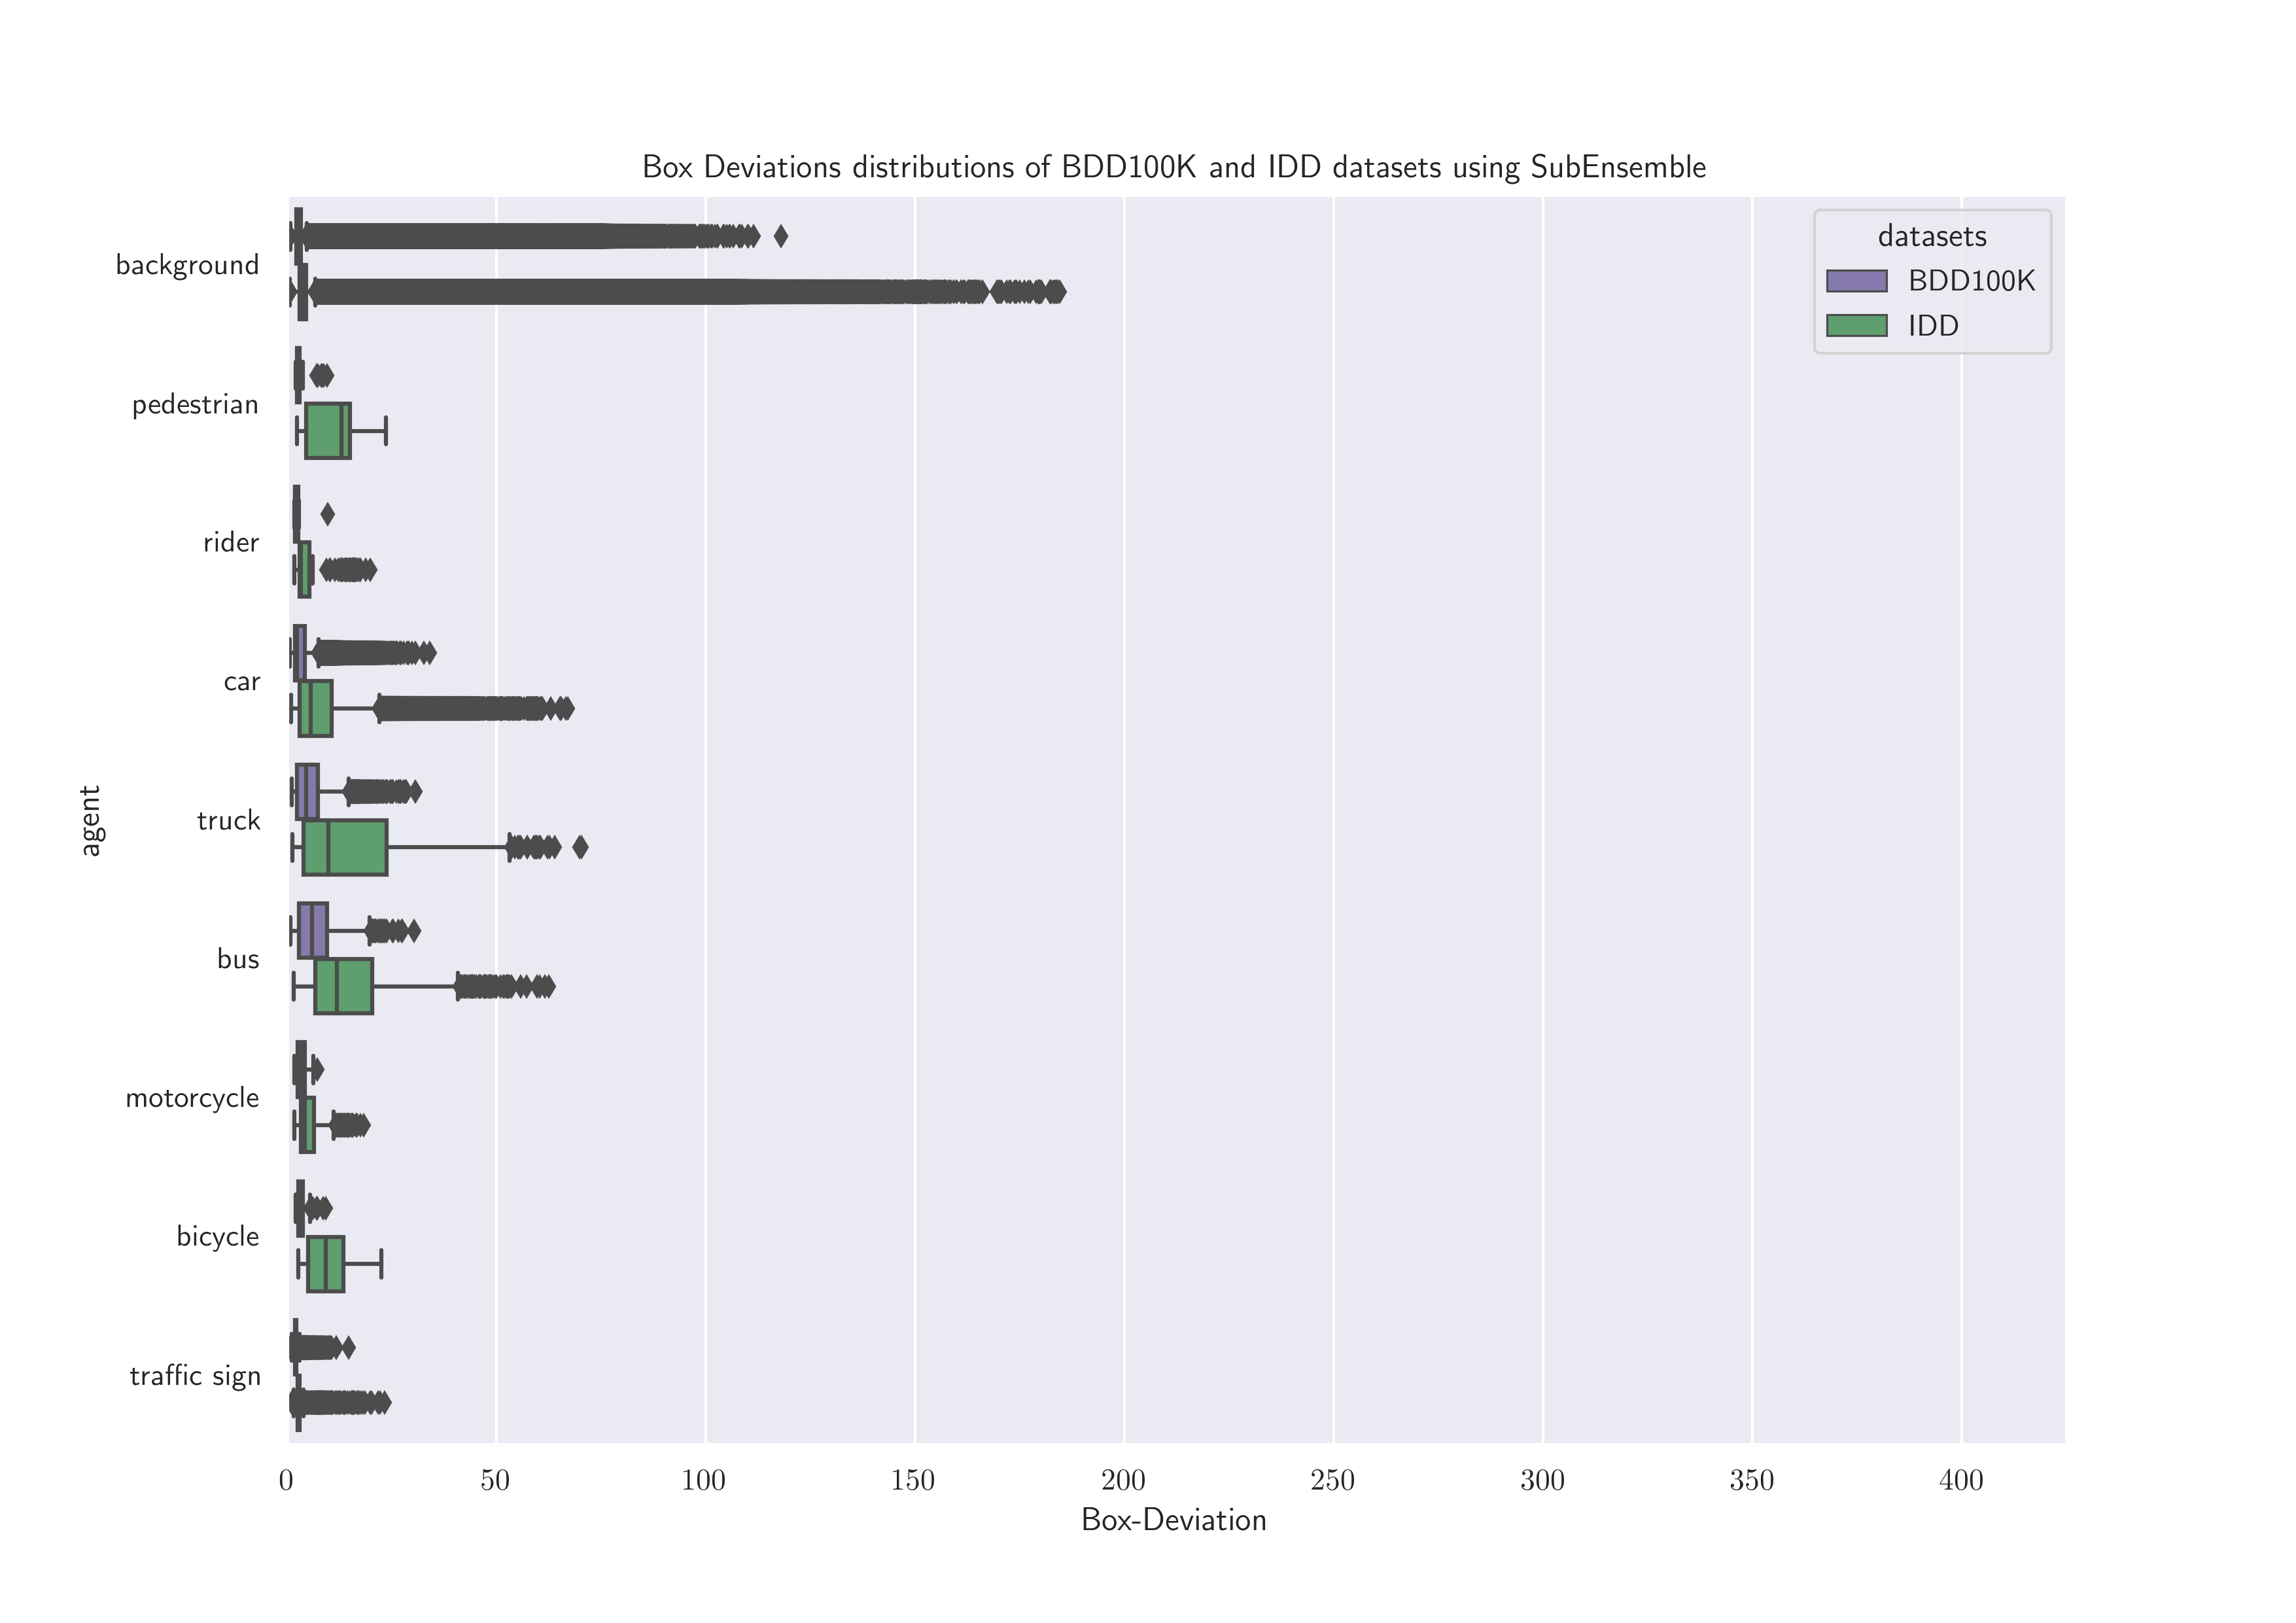
\includegraphics[scale=0.6]{images/distributions/SubEns_bdd_vs_iid_deviations.png}
        \caption[Box plot of box deviations with Sub-Ensemble model]{Box plot representing the summary of the entropy calculated from the mean of the softmax scores from multiple models of Sub-Ensemble.}
        \label{fig:subens_dev_summary}
    \end{figure}
    The previous works done by \citet{Feng2018, Feng2019} showed that one cause for box deviation is the result of objects getting occluded, but from the samples, we observed from the \acrshort{idd} dataset that standard deviation is also high in case of objects not being an exact match to the objects experienced during the training procedure. 
    % Since the equal scaling for both \acrshort{bnn} and Sub-Ensembles led to the unclear representation of deviation. We decided to use an independent scaling for both \acrshort{bnn} and Sub-Ensemble which represents the data deviation data more understandably. 
    
    % \begin{figure}
    %     \centering
    %     \includegraphics[scale=0.6]{images/distributions/BNN_bdd_vs_iid_deviations_1.png}
    %     \caption{Box plot representing the summary of the entropy calculated from the mean of the softmax scores from all the forward passes through the \acrshort{bnn}}
    %     \label{fig:bnn_dev_summary}
    % \end{figure}
    
    % \begin{figure}
    %     \centering
    %     \includegraphics[scale=0.6]{images/distributions/SubEns_bdd_vs_iid_deviations_1.png}
    %     \caption{Box plot representing the summary of the entropy calculated from the mean of the softmax scores from }
    %     \label{fig:subens_dev_summary}
    % \end{figure}
    
    \begin{figure}[H]
        \centering
        \begin{subfigure}[t]{\textwidth}
    		\centering
    		\includegraphics[scale=0.45]{images/detections/uncertainty_vis/UQ_gt_Viz.png}
    		\caption{Clear weather}
    		\label{clear_weather}
    	\end{subfigure}
    % \end{figure}
    % \begin{figure}[H] \ContinuedFloat
    	\begin{subfigure}[t]{\textwidth}
    		\centering
    		\includegraphics[scale=0.45]{images/detections/uncertainty_vis/UQ_gt_Viz_2.png}
    		\caption{Rainy weather}
    		\label{rainy_weather}
    	\end{subfigure}
        \caption[Detection on image from \acrshort{bdd} detection with uncertainty]{Detections made by SSD300 model on \acrshort{bdd} dataset and the uncertainties quantified using Sub-Ensemble based SSD model. The boxes in blue are the ground truth boxes and the boxes in other colors are the detection made. The bounding box label of the detection is (probability, class name, entropy) and the major axis of the ellipse in red represents the box deviation. From Figure \ref{clear_weather}, we can observe that detection of occluded cars are made with high variance. From Figure \ref{rainy_weather}, we can also observe that all detections are made with high variance.}
        \label{fig:uq_det_bdd}
    \end{figure}
    
    % \begin{figure}
    %     \centering
    %     \includegraphics[width=0.495\textwidth]{images/det_images/bdd_1.jpg}
    %     \includegraphics[width=0.495\textwidth]{images/det_images/bdd_bnn_entropies_1.png}
    %     \includegraphics[width=0.495\textwidth]{images/det_images/bdd_bnn_variances_1.png}
    %     \includegraphics[width=0.495\textwidth]{images/det_images/all_bnn_bdd_1.png}
    %     \caption{Caption}
    %     \label{fig:uq_observations}
    % \end{figure}
    
    \begin{figure}[H]
     \captionsetup[table]{skip=0pt}
    	\centering
    	\begin{subfigure}[t]{0.495\textwidth}
    		\centering
    		\includegraphics[width=\textwidth]{images/det_images/bdd_1.jpg}
    		\caption{Normal Detections}
    	\end{subfigure}
    	%
    	\begin{subfigure}[t]{0.495\textwidth}
    		\centering
    		\includegraphics[width=\textwidth]{images/det_images/bdd_bnn_entropies_1.png}
    		\caption{Detections with entropy encoded in box color}
    	\end{subfigure}
    % \end{figure}
    % \begin{figure}[H] \ContinuedFloat
    	\begin{subfigure}[t]{0.495\textwidth}
    		\centering
    		\includegraphics[width=\textwidth]{images/det_images/bdd_bnn_variances_1.png}
    		\caption{Detections with variances represented as ellipses}
    	\end{subfigure}
    	%
    	\begin{subfigure}[t]{0.495\textwidth}
    		\centering
    		\includegraphics[width=\textwidth]{images/det_images/all_bnn_bdd_1.png}
    		\caption{Visualizing all 8732 boxes regressed by SSD300}
    		\label{id_8732_boxes}
    	\end{subfigure}
    	
    	\begin{center}
    	    \begin{subfigure}[t]{0.495\textwidth}
    		\centering
    		\includegraphics[width=\textwidth]{images/Slide4.jpg}
    		\caption{Colormap representing the entropy to box color encoding}
    	\end{subfigure}
    	\label{bnn_inference_id}
    	\end{center}
    	
    	\caption[Bayesian SSd300 inference on image fro \acrshort{bdd}]{Inference of Bayesian-SSD300 model on a sample image from \acrshort{bdd}, including visualization of various uncertainty quantification metrics chose to perform \acrshort{ood} detection. Since the image chosen is from \acrshort{id} dataset, there is very little confusion in boxes regressed from the images as shown in Figure \ref{id_8732_boxes}. An entropy value of 0 implies that the model is very sure about the class assigned to the bounding box and a maximum value suggests that the model is very unsure about the class of the object present. The bounding box label of the detection is (probability, class name, entropy) and the major axis of the ellipse in red represents the box deviation.}
    	\label{uq_observations}
    \end{figure}
    
    \begin{figure}[H]
    	\centering
    	\begin{subfigure}[t]{0.495\textwidth}
    		\centering
    		\includegraphics[width=\textwidth]{images/det_images/idd_1.jpg}
    		\caption{Normal Detections}
    	\end{subfigure}
    	%
    	\begin{subfigure}[t]{0.495\textwidth}
    		\centering
    		\includegraphics[width=\textwidth]{images/det_images/idd_bnn_entropies_1.png}
    		\caption{Detections with entropy encoded in box color}
    	\end{subfigure}
    % \end{figure}
    % \begin{figure}[ht] \ContinuedFloat
    	\begin{subfigure}[t]{0.495\textwidth}
    		\centering
    		\includegraphics[width=\textwidth]{images/det_images/idd_bnn_variances_1.png}
    		\caption{Detections with variances represented as ellipses}
    	\end{subfigure}
    	%
    	\begin{subfigure}[t]{0.495\textwidth}
    		\centering
    		\includegraphics[width=\textwidth]{images/det_images/all_bnn_idd_0.png}
    		\caption{Visualizing all 8732 boxes regressed by SSD300}
    		\label{bnn_od_8732_boxes}
    	\end{subfigure}
    	
    	\caption[Bayesian SSD300 inference on image fro \acrshort{idd}]{Inference of Bayesian-SSD300 model on a sample image from \acrshort{idd} and visualization of various uncertainty quantification metrics chose to perform \acrshort{ood} detection. Since the image chosen is from \acrshort{ood} dataset, there is a lot confusion in boxes regressed from the images as shown in Figure \ref{bnn_od_8732_boxes}.The bounding box label of the detection is (probability, class name, entropy) and the major axis of the ellipse in red represents the box deviation.}
    	\label{bnn_inference_id_1}
    \end{figure}
    
    \begin{figure}[H]
    	\centering
    	\begin{subfigure}[t]{0.495\textwidth}
    		\centering
    		\includegraphics[width=\textwidth]{images/det_images/bdd_1.jpg}
    		\caption{Normal Detections}
    	\end{subfigure}
    	%
    	\begin{subfigure}[t]{0.495\textwidth}
    		\centering
    		\includegraphics[width=\textwidth]{images/det_images/bdd_subens_entropies_0.png}
    		\caption{Detections with entropy encoded in box color}
    	\end{subfigure}
    \end{figure}
    \begin{figure}[H] \ContinuedFloat
    	\begin{subfigure}[t]{0.495\textwidth}
    		\centering
    		\includegraphics[width=\textwidth]{images/det_images/subensemble_entropies_1.png}
    		\caption{Detections with variances represented as ellipses}
    	\end{subfigure}
    	%
    	\begin{subfigure}[t]{0.495\textwidth}
    		\centering
    		\includegraphics[width=\textwidth]{images/det_images/all_subens_bdd_1.png}
    		\caption{Visualizing all 8732 boxes regressed by SSD300}
    		\label{id_subens_8732_boxes}
    	\end{subfigure}
    	
    	\caption[Sub-Ensemble models inference on image from \acrshort{bdd} dataset]{Inference of Sub-Ensemble based SSD300 model and visualization of various uncertainty quantification metrics chose to perform \acrshort{ood} detection using . Since the image chosen is from \acrshort{id} dataset, there is very less confusion in boxes regressed from the images as shown in Figure \ref{id_subens_8732_boxes}. The bounding box label of the detection is (probability, class name, entropy) and the major axis of the ellipse in red represents the box deviation.}
    	\label{sens_inference_id}
    \end{figure}
    
    \begin{figure}[ht]
    	\centering
    	\begin{subfigure}[t]{0.495\textwidth}
    		\centering
    		\includegraphics[width=\textwidth]{images/det_images/idd_1.jpg}
    		\caption{Normal Detections}
    	\end{subfigure}
    	%
    	\begin{subfigure}[t]{0.495\textwidth}
    		\centering
    		\includegraphics[width=\textwidth]{images/det_images/subensemble_entropies_idd_1.png}
    		\caption{Detections with entropy encoded in box color}
    	\end{subfigure}
    % \end{figure}
    % \begin{figure}[H] \ContinuedFloat
    	\begin{subfigure}[t]{0.495\textwidth}
    		\centering
    		\includegraphics[width=\textwidth]{images/det_images/idd_subens_variances_1.png}
    		\caption{Detections with variances represented as ellipses}
    	\end{subfigure}
    	%
    	\begin{subfigure}[t]{0.495\textwidth}
    		\centering
    		\includegraphics[width=\textwidth]{images/det_images/all_subens_idd_0.png}
    		\caption{Visualizing all 8732 boxes regressed by SSD300}
    		\label{od_subens_8732_boxes}
    	\end{subfigure}
    	
    	\caption[Sub-Ensemble models inference on image from \acrshort{idd} dataset]{Inference of Sub-Ensemble based SSD300 model on an image sampled from \acrshort{ood} dataset and visualization of various uncertainty quantification metrics chose to perform \acrshort{ood} detection using Sub-Ensemble model. Since the image chosen is from \acrshort{ood} dataset, there is an inherent confusion in boxes regressed from the images as shown in Figure \ref{od_subens_8732_boxes}. The bounding box label of the detection is (probability, class name, entropy) and the major axis of the ellipse in red represents the box deviation.}
    	\label{sens_inference_oodd}
    \end{figure}
    
    From the experimental measurements and inference run visualization, it can be observed that:
    \begin{itemize}
        \item From Figure \ref{fig:uq_det_bdd} we can infer that box deviation is high in case of occlusions, this behavior can be observed clearly from the top image. The deviations are high in the case of cars' partial visibility even though the distance from the ego vehicle is small.
        \item In case of \acrshort{ood} sample a Van which is a subclass of Car superclass is assigned high entropy and box deviation.
        \item We also observed a peculiar behavior of standard deviation being high, if there is a change in weather condition from the weather conditions in training data.
        \item \acrshort{bnn} even though generated a best mAP score has struggled in providing plausible uncertainty values both in \acrshort{id} and \acrshort{ood} cases. This sort of behavior is visualized in Figures \ref{uq_observations} and \ref{bnn_inference_id_1}.
        \item Sub-Ensemble has performed well in quantifying uncertainty and also produced a good mAP score and only got outperformed by its Bayesian alternative.
    \end{itemize}
    
    \newpage

    \subsection{Out-of-Distribution Detection quantification using Uncertainty Quantification methods}
    \label{Exp:4}
    In this experiment, we use the information about Probability, Entropy and Box-Deviation obtained in the previous experiment to quantify their ability to perform \acrshort{ood} classification. We use the method proposed in Section \ref{benchmarking_metrics} to quantify the \acrshort{ood} classification ability. The metric we used to quantify the \acrshort{ood} ability is the \acrlong{auroc}.
    
    
    % Please add the following required packages to your document preamble:
    % \usepackage{multirow}
    \begin{table}[H]
        \centering
        \caption{\acrshort{auroc} scores representing the metrics ability obtained from different uncertainty quantification models}
        \label{tab:auroc_uq}
        \begin{tabular}{lllll}
            \hline
            \multicolumn{3}{l}{Models}                                               & Bayesian - SSD300 & \begin{tabular}[c]{@{}l@{}}Sub-Ensemble \\ SSD300\end{tabular} \\ \hline
            \multirow{30}{*}{Agents} & \multirow{3}{*}{Background}   & Probability   & 0.45              & 0.44                                                           \\ \cline{3-5} 
                                     &                               & Entropy       & 0.56              & 0.56                                                           \\ \cline{3-5} 
                                     &                               & Box-Deviation & \textbf{0.64}              & \textbf{0.75}                                                           \\ \cline{2-5} 
                                     & \multirow{3}{*}{Pedestrian}   & Probability   & 0.14              & 0.21                                                           \\ \cline{3-5} 
                                     &                               & Entropy       & 0.88              & 0.86                                                           \\ \cline{3-5} 
                                     &                               & Box-Deviation & \textbf{0.93}              & \textbf{0.95}                                                           \\ \cline{2-5} 
                                     & \multirow{3}{*}{Rider}        & Probability   & 0.75              & 0.34                                                           \\ \cline{3-5} 
                                     &                               & Entropy       & 0.59              & 0.72                                                           \\ \cline{3-5} 
                                     &                               & Box-Deviation & \textbf{0.82}              & \textbf{0.84}                                                           \\ \cline{2-5} 
                                     & \multirow{3}{*}{Car}          & Probability   & 0.45              & 0.46                                                           \\ \cline{3-5} 
                                     &                               & Entropy       & 0.59              & 0.58                                                           \\ \cline{3-5} 
                                     &                               & Box-Deviation & \textbf{0.76}              & \textbf{0.79}                                                           \\ \cline{2-5} 
                                     & \multirow{3}{*}{Truck}        & Probability   & 0.37              & 0.34                                                           \\ \cline{3-5} 
                                     &                               & Entropy       & 0.67              & 0.71                                                           \\ \cline{3-5} 
                                     &                               & Box-Deviation & \textbf{0.69}              & \textbf{0.74}                                                           \\ \cline{2-5} 
                                     & \multirow{3}{*}{Bus}          & Probability   & 0.38              & 0.4                                                            \\ \cline{3-5} 
                                     &                               & Entropy       & 0.64              & 0.62                                                           \\ \cline{3-5} 
                                     &                               & Box-Deviation & \textbf{0.7}               & \textbf{0.75}                                                           \\ \cline{2-5} 
                                     & \multirow{3}{*}{Motorcycle}   & Probability   & 0.49              & 0.53                                                           \\ \cline{3-5} 
                                     &                               & Entropy       & 0.6               & 0.51                                                           \\ \cline{3-5} 
                                     &                               & Box-Deviation & \textbf{0.62}              & \textbf{0.71}                                                           \\ \cline{2-5} 
                                     & \multirow{3}{*}{Bicycle}      & Probability   & 0.23              & 0.19                                                           \\ \cline{3-5} 
                                     &                               & Entropy       & 0.84              & 0.88                                                           \\ \cline{3-5} 
                                     &                               & Box-Deviation & \textbf{0.85}              & \textbf{0.94}                                                           \\ \cline{2-5} 
                                     & \multirow{3}{*}{Traffic Sign} & Probability   & \textbf{-}        & 0.41                                                           \\ \cline{3-5} 
                                     &                               & Entropy       & \textbf{-}        & 0.62                                                           \\ \cline{3-5} 
                                     &                               & Box-Deviation & \textbf{-}        & \textbf{0.88}                                                           \\ \cline{2-5} 
                                     & \multirow{3}{*}{All Classes}  & Probability   & 0.45              & 0.44                                                           \\ \cline{3-5} 
                                     &                               & Entropy       & 0.56              & 0.56                                                           \\ \cline{3-5} 
                                     &                               & Box-Deviation & \textbf{0.64}              & \textbf{0.75}                                                           \\ \hline
        \end{tabular}
    \end{table}
    
    \begin{figure}[ht]
    	\centering
    	\begin{subfigure}[t]{0.495\textwidth}
    		\centering
    		\includegraphics[width=\textwidth]{images/ROC/all classes_ROC_bdd_vs_idd_Score_using_bnn.pdf}
    		\caption{\acrshort{bnn}}
    	\end{subfigure}
    	%
    	\begin{subfigure}[t]{0.495\textwidth}
    		\centering
    		\includegraphics[width=\textwidth]{images/ROC/all classes_ROC_bdd_vs_idd_Score_using_subens.pdf}
    		\caption{Sub-Ensemble}
    	\end{subfigure}
    	\caption[ROC curves of \acrshort{ood} sample classification using uncertainty quantification methods]{Graphs visualizing the \acrshort{roc} curves representing the ability of \acrshort{ood} detection using \acrshort{bnn} and Sub-Ensemble based uncertainty quantification methods}
    	\label{uq_roc_curves}
    \end{figure}
    
    From the graphs shown in Figure \ref{uq_roc_curves}, we can conclude that the Sub-Ensemble model with standard deviation metric out-performed all the other methods by a large margin.
    As already mentioned in Section \ref{Benchmarking}, the \acrshort{ood} dataset consists of various inter and intra-class variances in between them. Hence, it is very important to understand the performance of each uncertainty quantification model at each class level. To address this requirement, we used the per-class metrics to classify \acrshort{id} and \acrshort{ood} data and to quantification of this ability is shown in Table \ref{tab:auroc_uq} and Figures \ref{fig:roc_bnn} and \ref{fig:roc_subens}. 
    
    \subsubsection{Observations}
    \begin{itemize}
        \item All the metrics struggled in classifying background class between \acrshort{id} and \acrshort{ood} data. But Sub-Ensemble model detected \acrshort{ood} backgrounds representing that backgrounds does not match exactly because the data is collected in different countries.
        \item Entropy and Box deviation performed well in detecting \acrshort{ood} samples using both Bayesian and Sub-Ensemble model. Box deviation also performed well in this case.
        \item In case of Rider class, entropy struggled to detect because of the inherent ambiguity in between \acrshort{id} and \acrshort{ood} samples. But box deviation had performed well in classifying between \acrshort{bdd} and \acrshort{idd} dataset.
        \item The performance of uncertainty quantification methods with Car, Truck and Bus classes is similar to that of Rider due to the inherent ambiguity between these classes in \acrshort{bdd} and \acrshort{idd} datasets.
        \item Entropy and Box deviation had performed well in case of Bicycle class in both the methods.
        \item Overall, box deviation had outperformed entropy in classifying samples from \acrshort{bdd} dataset to \acrshort{idd} dataset.
    \end{itemize}
    
    \begin{figure}[H]
    	\centering
    	\begin{subfigure}[t]{0.495\textwidth}
    		\centering
    		\includegraphics[width=\textwidth]{images/ROC/background_ROC_bdd_vs_idd_Score_using_bnn.pdf}
    		\caption{Background}
    	\end{subfigure}
    	%
    	\begin{subfigure}[t]{0.495\textwidth}
    		\centering
    		\includegraphics[width=\textwidth]{images/ROC/pedestrian_ROC_bdd_vs_idd_Score_using_bnn.pdf}
    		\caption{Pedestrian}
    	\end{subfigure}
    	
    	\begin{subfigure}[t]{0.495\textwidth}
    		\centering
    		\includegraphics[width=\textwidth]{images/ROC/rider_ROC_bdd_vs_idd_Score_using_bnn.pdf}
    		\caption{Rider}
    	\end{subfigure}
        %
    	\begin{subfigure}[t]{0.495\textwidth}
    		\centering
    		\includegraphics[width=\textwidth]{images/ROC/car_ROC_bdd_vs_idd_Score_using_bnn.pdf}
    		\caption{Car}
    	\end{subfigure}
    	
    	\begin{subfigure}[t]{0.495\textwidth}
    		\centering
    		\includegraphics[width=\textwidth]{images/ROC/truck_ROC_bdd_vs_idd_Score_using_bnn.pdf}
    		\caption{Truck}
    	\end{subfigure}
        %
    	\begin{subfigure}[t]{0.495\textwidth}
    		\centering
    		\includegraphics[width=\textwidth]{images/ROC/bus_ROC_bdd_vs_idd_Score_using_bnn.pdf}
    		\caption{Bus}
    	\end{subfigure}
    	\end{figure}
        	
    \begin{figure} \ContinuedFloat
    
    	\begin{subfigure}[t]{0.495\textwidth}
    		\centering
    		\includegraphics[width=\textwidth]{images/ROC/motorcycle_ROC_bdd_vs_idd_Score_using_bnn.pdf}
    		\caption{Motorcycle}
    	\end{subfigure}
        %
    	\begin{subfigure}[t]{0.495\textwidth}
    		\centering
    		\includegraphics[width=\textwidth]{images/ROC/bicycle_ROC_bdd_vs_idd_Score_using_bnn.pdf}
    		\caption{Bicycle}
    	\end{subfigure}
        \vspace*{-3mm}
        \caption[Class-wise ROC curves for \acrshort{ood} sample classification using uncertainty quantification metrics with \acrshort{bnn}]{\acrlong{roc} curves for each class in \acrshort{bdd} dataset using Bayesian-SSD300 model}
        \label{fig:roc_bnn}
    \end{figure}


     \begin{figure}[H]
    	\centering
    	\begin{subfigure}[t]{0.495\textwidth}
    		\centering
    		\includegraphics[width=\textwidth]{images/ROC/background_ROC_bdd_vs_idd_Score_using_subens.pdf}
    		\caption{Background}
    	\end{subfigure}
    	%
    	\begin{subfigure}[t]{0.495\textwidth}
    		\centering
    		\includegraphics[width=\textwidth]{images/ROC/pedestrian_ROC_bdd_vs_idd_Score_using_subens.pdf}
    		\caption{Pedestrian}
    	\end{subfigure}
    	
    	\begin{subfigure}[t]{0.495\textwidth}
    		\centering
    		\includegraphics[width=\textwidth]{images/ROC/rider_ROC_bdd_vs_idd_Score_using_subens.pdf}
    		\caption{Rider}
    	\end{subfigure}
        %
    	\begin{subfigure}[t]{0.495\textwidth}
    		\centering
    		\includegraphics[width=\textwidth]{images/ROC/car_ROC_bdd_vs_idd_Score_using_subens.pdf}
    		\caption{Car}
    	\end{subfigure}
    	\end{figure}
        	
    \begin{figure}[H] \ContinuedFloat
    	\begin{subfigure}[t]{0.495\textwidth}
    		\centering
    		\includegraphics[width=\textwidth]{images/ROC/truck_ROC_bdd_vs_idd_Score_using_subens.pdf}
    		\caption{Truck}
    	\end{subfigure}
        %
    	\begin{subfigure}[t]{0.495\textwidth}
    		\centering
    		\includegraphics[width=\textwidth]{images/ROC/bus_ROC_bdd_vs_idd_Score_using_subens.pdf}
    		\caption{Bus}
    	\end{subfigure}
        
    	\begin{subfigure}[t]{0.495\textwidth}
    		\centering
    		\includegraphics[width=\textwidth]{images/ROC/motorcycle_ROC_bdd_vs_idd_Score_using_subens.pdf}
    		\caption{Motorcycle}
    	\end{subfigure}
        %
    	\begin{subfigure}[t]{0.495\textwidth}
    		\centering
    		\includegraphics[width=\textwidth]{images/ROC/bicycle_ROC_bdd_vs_idd_Score_using_subens.pdf}
    		\caption{Bicycle}
    	\end{subfigure}
    % 	\end{figure}
        	
    % \begin{figure}[H]\ContinuedFloat
    	
    	\begin{center}
    	\begin{subfigure}[t]{0.495\textwidth}
    		\centering
    		\includegraphics[width=\textwidth]{images/ROC/traffic sign_ROC_bdd_vs_idd_Score_using_subens.pdf}
    		\caption{Traffic Sign}
    	\end{subfigure}
    	\end{center}
        \vspace*{-3mm}
        \caption[Class-wise ROC curves for \acrshort{ood} sample classification using uncertainty quantification metrics with Sub-Ensemble models]{\acrlong{roc} curves for each class in \acrshort{bdd} dataset using SubEnsemble-SSD300 model}
        \label{fig:roc_subens}
    \end{figure}
    
    
    
    % \subsubsection{Visualizations}
    
    % \begin{figure}[H]
    % 	\centering
    % 	\captionsetup[figure]{font=small,skip=0pt}
    % 	\begin{subfigure}[t]{0.495\textwidth}
    % 		\centering
    % 		\includegraphics[width=\textwidth]{images/uq_viz/BNN/bdd/without_background/8_detected.png}
    % 		\caption{\acrshort{bdd} - without background}
    % 	\end{subfigure}
    % 	%
    % 	\begin{subfigure}[t]{0.495\textwidth}
    % 		\centering
    % 		\includegraphics[width=\textwidth]{images/uq_viz/BNN/bdd/with_background/8_detected.png}
    % 		\caption{\acrshort{bdd} - with background}
    % 	\end{subfigure}
    % \end{figure}
    % \begin{figure} \ContinuedFloat	
    % 	\begin{subfigure}[t]{0.495\textwidth}
    % 		\centering
    % 		\includegraphics[width=\textwidth]{images/uq_viz/BNN/idd/without_background/6_detected.png}
    % 		\caption{\acrshort{idd} - without background}
    % 	\end{subfigure}
    % 	%
    % 	\begin{subfigure}[t]{0.495\textwidth}
    % 		\centering
    % 		\includegraphics[width=\textwidth]{images/uq_viz/BNN/idd/with_background/6_detected.png}
    % 		\caption{\acrshort{idd} - with background}
    % 	\end{subfigure}
    	
    % 	\begin{center}
    % 	    \begin{subfigure}[t]{0.495\textwidth}
    % 		\centering
    % 		\includegraphics[width=\textwidth]{images/Slide4.jpg}
    % 		\caption{Colormap for box color encoding}
    % 	\end{subfigure}
    % 	\end{center}
    	
    % 	\caption{Image with the detections performed using \acrshort{bnn} the boxes in Image (a) and Image (c) are the boxes without applying \acrshort{nms} and the box color information encodes the uncertainty information. The colormap provides the correspondence between the color of the bounding box and the entropy.}
    % 	\label{uq_weather_roc_curves}
    % \end{figure}
    
    % \begin{figure}[H]
    %     \label{\ref{Exp:5}}
    % 	\centering
    % 	\begin{subfigure}[t]{0.495\textwidth}
    % 		\centering
    % 		\includegraphics[width=\textwidth]{images/uq_viz/SubEns/bdd/without_background/8_detected.png}
    % 		\caption{\acrshort{bdd} - without background}
    % 	\end{subfigure}
    % 	%
    % 	\begin{subfigure}[t]{0.495\textwidth}
    % 		\centering
    % 		\includegraphics[width=\textwidth]{images/uq_viz/SubEns/bdd/with_background/8_detected.png}
    % 		\caption{\acrshort{bdd} - with background}
    % 	\end{subfigure}
    	
    % 	\begin{subfigure}[t]{0.495\textwidth}
    % 		\centering
    % 		\includegraphics[width=\textwidth]{images/uq_viz/SubEns/idd/without_background/6_detected.png}
    % 		\caption{\acrshort{idd} - without background}
    % 	\end{subfigure}
    % 	%
    % 	\begin{subfigure}[t]{0.495\textwidth}
    % 		\centering
    % 		\includegraphics[width=\textwidth]{images/uq_viz/SubEns/idd/with_background/6_detected.png}
    % 		\caption{\acrshort{idd} - with background}
    % 	\end{subfigure}
    	
    % 	\caption{Image with the detections performed using SubEnsemble. the boxes in Image (a) and Image (c) are the boxes without applying \acrshort{nms} and the box color information encodes the uncertainty information}
    % 	\label{uq_weather_roc_curves}
    % \end{figure}
    \newpage
    \subsection{\acrlong{ood} Detection with \acrshort{bdd}-Weather dataset}
    \label{Exp:5}
    This experiment is performed to quantify the ability of uncertainty quantification methods in classifying \acrshort{bdd} dataset and \acrshort{bdd}-weather dataset which is part of the $OD^2$ dataset proposed in Section \ref{bdd100k_weather}. We followed the same procedure as the previous experiments as outlined in Section \ref{benchmarking_metrics}. 

    To understand the effectiveness of these methods with the different weather conditions, we evaluated the \acrshort{ood} detection ability in different weather conditions. The following graphs provide the quantification of the \acrshort{ood} detection ability
    
    \begin{table}[H]
        \centering
        \caption{Uncertainty quantification metrics calculated using Bayesian and Sub-Ensemble versions of SSD300 model. The scores suggest that uncertainty based \acrshort{ood} detectors are not effective in detecting \acrshort{ood} samples.}
        \label{tab:my-table}
        \begin{tabular}{llll}
            \hline
                      &               & \begin{tabular}[c]{@{}l@{}}Bayesian\\ SSD300\end{tabular} & \begin{tabular}[c]{@{}l@{}}Sub-Ensemble\\ SSD300\end{tabular} \\ \hline
            Flood     & Probability   & 0.43            & 0.5                                                           \\ \hline
                      & Entropy       & \textbf{0.57}            & 0.5                                                           \\ \hline
                      & Box Deviation & 0.46            & 0.5                                                           \\ \hline
            Smog      & Probability   & 0.43            & 0.5                                                           \\ \hline
                      & Entropy       & \textbf{0.57}            & 0.5                                                           \\ \hline
                      & Box Deviation & 0.44            & 0.5                                                           \\ \hline
            Wild Fire & Probability   & \textbf{0.51}            & \textbf{0.53}                                                          \\ \hline
                      & Entropy       & 0.49            & 0.46                                                          \\ \hline
                      & Box Deviation & 0.49            & 0.46                                                          \\ \hline
        \end{tabular}
    \end{table}
    
    \begin{figure}[H]
    	\centering
    	\begin{subfigure}[t]{0.495\textwidth}
    		\centering
    		\includegraphics[width=\textwidth]{images/weather_roc/normal vs flood_ROC_Score_using_bnn.pdf}
    		\caption{Flood}
    	\end{subfigure}
    	%
    	\begin{subfigure}[t]{0.495\textwidth}
    		\centering
    		\includegraphics[width=\textwidth]{images/weather_roc/normal vs smog_ROC_Score_using_bnn.pdf}
    		\caption{Smog}
    	\end{subfigure}
    \end{figure}
    \begin{figure}[H] \ContinuedFloat
    	\begin{center}
    	\begin{subfigure}[t]{0.495\textwidth}
    		\centering
    		\includegraphics[width=\textwidth]{images/weather_roc/normal vs wildfire_ROC_Score_using_bnn.pdf}
    		\caption{Wild-Fire}
    	\end{subfigure}
    	\end{center}
    	\caption[ROC curves of weather \acrshort{ood} detection using \acrshort{bnn}]{Graphs visualizing the \acrshort{roc} curves representing the ability of \acrshort{ood} detection with \acrshort{bdd}-Weather using \acrshort{bnn}}
    	\label{uq_weather_roc_curves}
    \end{figure}
    
    \begin{figure}[ht]
    	\centering
    	\begin{subfigure}[t]{0.495\textwidth}
    		\centering
    		\includegraphics[width=\textwidth]{images/weather_roc/normal vs flood_ROC_Score_using_subens.pdf}
    		\caption{Flood}
    	\end{subfigure}
    	%
    	\begin{subfigure}[t]{0.495\textwidth}
    		\centering
    		\includegraphics[width=\textwidth]{images/weather_roc/normal vs smog_ROC_Score_using_subens.pdf}
    		\caption{Smog}
    	\end{subfigure}
    % \end{figure}
    % \begin{figure} \ContinuedFloat
    	\begin{center}
    	\begin{subfigure}[t]{0.495\textwidth}
    		\centering
    		\includegraphics[width=\textwidth]{images/weather_roc/normal vs wildfire_ROC_Score_using_subens.pdf}
    		\caption{Wild-Fire}
    	\end{subfigure}
    	\end{center}
    	\caption[ROC curves of weather \acrshort{ood} detection using Sub-Ensembles]{Graphs visualizing the \acrshort{roc} curves representing the ability of \acrshort{ood} detection with \acrshort{bdd}-Weather using Sub-Ensembles}
    	\label{uq_weather_roc_curves}
    \end{figure}
    
    \begin{figure}[ht]
        \captionsetup[subfigure]{labelformat=empty}
        \begin{tabular}{cccc}
            \subfloat{\includegraphics[width = 1.4in]{images/uq_weathers/BNN_entropies2.png}} &
            \subfloat{\includegraphics[width = 1.4in]{images/uq_weathers/BNN_entropies1.png}} &
            \subfloat{\includegraphics[width = 1.4in]{images/uq_weathers/BNN_entropies3.png}} &
            \subfloat{\includegraphics[width = 1.4in]{images/uq_weathers/BNN_entropies4.png}}\\
            \subfloat{\includegraphics[width = 1.4in]{images/uq_weathers/BNN_variances2.png}} &
            \subfloat{\includegraphics[width = 1.4in]{images/uq_weathers/BNN_variances1.png}} &
            \subfloat{\includegraphics[width = 1.4in]{images/uq_weathers/BNN_variances3.png}} &
            \subfloat{\includegraphics[width = 1.4in]{images/uq_weathers/BNN_variances4.png}}\\
            \subfloat[Normal Weather]{\includegraphics[width = 1.4in]{images/uq_weathers/flipout_entropies_all2.png}} &
            \subfloat[Flood]{\includegraphics[width = 1.4in]{images/uq_weathers/flipout_entropies_all1.png}} &
            \subfloat[Smog]{\includegraphics[width = 1.4in]{images/uq_weathers/flipout_entropies_all3.png}} &
            \subfloat[Wild Fire]{\includegraphics[width = 1.4in]{images/uq_weathers/flipout_entropies_all4.png}}\\
        \end{tabular}
        \caption[Detection on an image from \acrshort{bdd-c} dataset using \acrshort{bnn}]{Detection and entropy visualization on a randomly sampled image from the \acrshort{bdd-c} dataset using \acrshort{bnn}. We can observe that the model struggled in detecting objects as weather intensity increases. Also we can observe that there are lot less detection boxes seen compared to un-changed input image. The all boxes figure shows that majority of the boxes belong to background}
        \label{Flipout_uq_det}
    \end{figure}
    
    \begin{figure}[ht]
        \captionsetup[subfigure]{labelformat=empty}
        \begin{tabular}{cccc}
            \subfloat{\includegraphics[width = 1.4in]{images/uq_weathers/SubEns_entropies2.png}} &
            \subfloat{\includegraphics[width = 1.4in]{images/uq_weathers/SubEns_entropies1.png}} &
            \subfloat{\includegraphics[width = 1.4in]{images/uq_weathers/SubEns_entropies3.png}} &
            \subfloat{\includegraphics[width = 1.4in]{images/uq_weathers/SubEns_entropies4.png}}\\
            \subfloat{\includegraphics[width = 1.4in]{images/uq_weathers/SubEns_Variance2.png}} &
            \subfloat{\includegraphics[width = 1.4in]{images/uq_weathers/SubEns_Variance1.png}} &
            \subfloat{\includegraphics[width = 1.4in]{images/uq_weathers/SubEns_Variance3.png}} &
            \subfloat{\includegraphics[width = 1.4in]{images/uq_weathers/SubEns_Variance4.png}}\\
            \subfloat[Normal Weather]{\includegraphics[width = 1.4in]{images/uq_weathers/SubEns_entropies_all2.png}} &
            \subfloat[Flood]{\includegraphics[width = 1.4in]{images/uq_weathers/SubEns_entropies_all1.png}} &
            \subfloat[Smog]{\includegraphics[width = 1.4in]{images/uq_weathers/SubEns_entropies_all3.png}} &
            \subfloat[Wild Fire]{\includegraphics[width = 1.4in]{images/uq_weathers/SubEns_entropies_all4.png}}\\
        \end{tabular}
        \caption[Detection on an image from \acrshort{bdd-c} dataset using Sub-Ensembles]{Detection and entropy visualization on a randomly sampled image from the \acrshort{bdd-c} dataset using Sub-Ensembles. We observed a similar kind of box regression behavior to \acrshort{bnn} with sub-ensembles}
        \label{SubEns_uq_det}
    \end{figure}
    Figures \ref{Flipout_uq_det} and \ref{SubEns_uq_det} shows different images from different weathers placed column-wise with different metrics arranged row-wise. From these figures, we can observe that the weather condition neutralizes the variance as it makes all the samples ambiguous resulting in making entropy not useful for \acrshort{ood} detection. 
    \subsubsection{Observations}
    \begin{itemize}
        \item The uncertainty quantification based \acrshort{ood} detection methods are not effective for detecting \acrshort{ood} data due to change in weather conditions.
        \item We observed that with change in weather the object detection performance has deteriorated especially in the case of flood images.
        \item The entropy visualizations suggest that the model is very confident on Smog dataset that un-modified dataset. This behavior needs to be further analyzed to extract a more plausible understanding of using entropy for \acrshort{ood} detection.   
        \item The \acrshort{auroc} scores suggest that using uncertainty quantification methods performed almost similar to an unbiased random classifier.
        \item \acrshort{bnn} based uncertainty quantification could detect \acrshort{ood} data due to the object present in \acrshort{bdd}-Weather dataset is not ambiguous compared to the training dataset.
        \item The reason for the uncertainty quantification methods not being able to detect skewed datasets complies with the results reported by \citet{Ovadia2019}. The authors performed their experiments on the classification dataset and showed that the entropy measured doesn't differentiate \acrshort{id} samples and their corresponding skewed samples.
    \end{itemize}
    
\end{document}
